%% ****** Start of file apstemplate.tex ****** %
%%
%%
%%   This file is part of the APS files in the REVTeX 4 distribution.
%%   Version 4.1r of REVTeX, August 2010
%%
%%
%%   Copyright (c) 2001, 2009, 2010 The American Physical Society.
%%
%%   See the REVTeX 4 README file for restrictions and more information.
%%
%
% This is a template for producing manuscripts for use with REVTEX 4.0
% Copy this file to another name and then work on that file.
% That way, you always have this original template file to use.
%
% Group addresses by affiliation; use superscriptaddress for long
% author lists, or if there are many overlapping affiliations.
% For Phys. Rev. appearance, change preprint to twocolumn.
% Choose pra, prb, prc, prd, pre, prl, prstab, prstper, or rmp for journal
%  Add 'draft' option to mark overfull boxes with black boxes
%  Add 'showpacs' option to make PACS codes appear
%  Add 'showkeys' option to make keywords appear
\documentclass[aps,pre,reprint,superscriptaddress, twocolumn]{revtex4}
%\documentclass[aps,pre,preprint,superscriptaddress]{revtex4}
%\documentclass[aps,prl,reprint,groupedaddress]{revtex4}

% You should use BibTeX and apsrev.bst for references
% Choosing a journal automatically selects the correct APS
% BibTeX style file (bst file), so only uncomment the line
% below if necessary.
\bibliographystyle{apsrev4-1}

\usepackage{graphicx}
\usepackage{amsmath}
\usepackage{float}

\newcommand{\e}[1]{\times10^{#1}}
\newcommand{\gd}{\dot{\gamma}}
\newcommand{\com}[1]{{\bf {#1}}}

\begin{document}

% Use the \preprint command to place your local institutional report
% number in the upper righthand corner of the title page in preprint mode.
% Multiple \preprint commands are allowed.
% Use the 'preprintnumbers' class option to override journal defaults
% to display numbers if necessary
%\preprint{}

%Title of paper
\title{Rheology of Cubic Blue Phases}

% repeat the \author .. \affiliation  etc. as needed
% \email, \thanks, \homepage, \altaffiliation all apply to the current
% author. Explanatory text should go in the []'s, actual e-mail
% address or url should go in the {}'s for \email and \homepage.
% Please use the appropriate macro foreach each type of information

% \affiliation command applies to all authors since the last
% \affiliation command. The \affiliation command should follow the
% other information
% \affiliation can be followed by \email, \homepage, \thanks as well.

\author{O. Henrich}
\email[Corresponding author: ]{o.henrich@ucl.ac.uk}
\affiliation{EPCC, School of Physics and Astronomy, University of Edinburgh,\\JCMB Kings Buildings, Mayfield Road, Edinburgh EH9 3JZ, UK}
\affiliation{Centre for Computational Science, University College London,\\20 Gordon Street, London WC1H 0AJ, UK}

\author{K. Stratford}
\affiliation{EPCC, School of Physics and Astronomy, University of Edinburgh,\\JCMB Kings Buildings, Mayfield Road, Edinburgh EH9 3JZ, UK}

\author{P.V. Coveney}
\affiliation{Centre for Computational Science, University College London,\\20 Gordon Street, London WC1H 0AJ, UK}

\author{M.E. Cates}
\affiliation{SUPA, School of Physics and Astronomy, University of Edinburgh,\\JCMB Kings Buildings, Mayfield Road, Edinburgh EH9 3JZ, UK}

\author{D. Marenduzzo}
\affiliation{SUPA, School of Physics and Astronomy, University of Edinburgh,\\JCMB Kings Buildings, Mayfield Road, Edinburgh EH9 3JZ, UK}


%\homepage[]{Your web page}
%\thanks{}
%\altaffiliation{}

%Collaboration name if desired (requires use of superscriptaddress
%option in \documentclass). \noaffiliation is required (may also be
%used with the \author command).
%\collaboration can be followed by \email, \homepage, \thanks as well.
%\collaboration{}

%\noaffiliation

\date{\today}

\begin{abstract}
We study the behaviour of cubic blue phases under shear flow
via lattice Boltzmann simulations. We focus on the two experimentally observed
phases, Blue Phase I (BPI) and Blue Phase II (BPII). The disclination network of Blue Phase 
II continuously breaks and reforms under shear, leading to an oscillatory stress response in time.
\end{abstract}

% insert suggested PACS numbers in braces on next line
\pacs{47.11.Qr, 47.57.Lj, 47.57.Qk, 61.30.Dk, 61.30.Pq, 61.30.Jf, 83.80.Xz}
% insert suggested keywords - APS authors don't need to do this
\keywords{blue phase, cholesterics, chiral nematics, rheology}

%\maketitle must follow title, authors, abstract, \pacs, and \keywords
\maketitle

% body of paper here - Use proper section commands
% References should be done using the \cite, \ref, and \label commands
\section{Introduction}
% Put \label in argument of \section for cross-referencing
%\section{\label{}}

Cholesterics are liquid crystals in which the local nematic director field spontaneously 
twists in thermodynamic equilibrium~\cite{deGennes}. The preferred configuration close 
to the isotropic boundary features twist around two perpendicular axes, as opposed to 
just one axis in the regular cholesteric state, and the corresponding deformation is 
denoted a ``double-twist cylinder''.
As it is topologically impossible to cover continuously 3D space with double-twist 
cylinders, defects arise. These organise into a variety of regular periodic lattices, 
giving rise to the so-called cubic blue phases (BPs)~\cite{Grebel:1984,Wright:1989}. 
There are two experimentally observed cubic blue phases, BPI and BPII (a third, BPIII, 
is thought to be amorphous~\cite{Henrich:2011a}).

BPs have been long considered as purely of academic interest due to their very narrow 
range of stability. This view has changed since the creation of polymer-stabilised and 
temperature-stabilised BPs~\cite{Kikuchi:2002,Coles:2005}, which has opened up the 
possibility of novel applications.
During the last few years considerable progress has been achieved regarding the behaviour 
of BPs in confined geometries~\cite{Fukuda:2010a, Fukuda:2010b, Ravnik:2011b}, under 
external fields ~\cite{Alexander:2008,Fukuda:2009,Henrich:2010a,Castles:2010,Tiribocchi:2011a}, 
and in the presence of colloidal particles~\cite{Ravnik:2011a}.
The kinetics of BP domain growth have been recently addressed in~\cite{Henrich:2010b}. 
However, our understanding of their dynamical behaviour under flow remains
very limited. The aim of this work is to address this issue by studying,
for the first time, the response of confined BP samples to a shear flow.

Flow response in cholesterics is both strongly non-Newtonian and highly anisotropic.
For example, if a cholesteric helix is subjected to a Poiseuille flow along
the helical axis, small pressure differences drive flow mainly through
''permeation'', first investigated by Helfrich~\cite{Helfrich:1969}.
In the permeation mode the liquid crystal flows while leaving the director
field virtually unchanged, which leads to high dissipation and large
viscosities. Marenduzzo et al.~\cite{Marenduzzo:2006a,Marenduzzo:2006b} simulated 
shear and Poiseuille flow in cholesteric liquid crystals in the permeation mode, and 
showed the importance of the boundary conditions in determining the apparent viscosity of the fluid. 
They also found that a strong secondary flow appears.
Rey~\cite{Rey:1996a, Rey:1996b} studied shear in cholesterics oriented with the helix along 
the vorticity axis and found that, at low Ericksen number, travelling twist waves appear which 
lead to the rotation of the cholesteric helix. At higher forcing, the helix uncoils and 
leaves a flow-induced nematic phase.
Rey also studied cholesterics subjected to both steady flow and low frequency
small amplitude oscillatory shear for different helix orientations
~\cite{Rey:2000, Rey:2002}. He found that splay/bend/twist deformations were
excited when the helix was aligned along the flow direction; splay/bend
deformation occurred when the helix was aligned along the velocity gradient;
but only twist deformations
appeared when the helix was aligned along the vorticity axis.

Dupuis et al.~\cite{Dupuis:2005} performed the first numerical investigation of BP rheology 
in Poiseuille flow, starting from equilibrium structures of BPI and BPII and a periodic 
array of doubly twisted cylinders.
Under small forcing, the network opposed the flow giving rise to a significant 
increase in apparent viscosity.
Upon increasing the forcing they found clear evidence of shear thinning.
In the crossover region they predicted a novel oscillatory regime where the network 
continuously breaks and reforms as portions of the disclinations in the centre of the channel 
move to neighbouring cells and relink with the parts of the network left behind by the flow. 
Compared with the cholesteric case, the viscosity still decreases with forcing 
(the system shear thins) but much less than
for cholesterics in the permeation mode, which is in agreement with experiments
~\cite{Zapotocky:1999, Ramos:2002}.

\section{Model and Methods}

Our approach is based on the well-established Beris-Edwards model for hydrodynamics of
cholesteric liquid crystals \cite{Beris:1994}, which describes the ordered state 
in terms of a traceless, symmetric tensor order parameter ${\mathbf Q}({\mathbf r})$. 
In the uniaxial approximation, the order parameter is given by
$Q_{\alpha \beta}= q_s ( \hat{n}_\alpha \hat{n}_\beta - \frac{1}{3}\; \delta_{\alpha\beta})$
with $\hat{{\mathbf n}}$ the director field and $q_s$ the amplitude of nematic
order. More generally,
the largest eigenvalue of ${\mathbf Q}$, $0\le q_s\le\frac{2}{3}$
characterises the local degree of orientational order.
The thermodynamic properties of the liquid crystal are determined by a free energy
${\cal F}$, whose density $f$ consists of a bulk contribution $f_b$ and a gradient part $f_g$, as follows,
\begin{eqnarray}
f_b&=&\frac{A_0}{2}\left(1-\frac{\gamma}{3}\right) Q_{\alpha \beta}^2\nonumber\\
&-&\frac{A_0 \gamma}{3}Q_{\alpha \beta} Q_{\beta \gamma} Q_{\gamma \alpha}+\frac{A_0 \gamma}{4}(Q_{\alpha \beta}^2)^2,\nonumber\\
f_g&=&\frac{K}{2}(\varepsilon_{\alpha\gamma\delta} \partial_\gamma Q_{\delta\beta}+2 q_0 Q_{\alpha \beta})^2+\frac{K}{2}(\partial_\beta Q_{\alpha \beta})^2.\label{FE}
\end{eqnarray}
The first term contains the bulk-free energy constant $A_0$ and the inverse temperature $\gamma$ which controls the magnitude of order.
The second part quantifies the cost of elastic distortions, which are proportional to the elastic constant $K$;
we work for simplicity in the one-elastic constant approximation. The wavevector $q_0=2\pi/p_0$, where $p_0$ is the cholesteric pitch.
The actual periodicity of the BP structure, $p$, does not need to be equal to $p_0$.
The ``redshift'' $r=p/p_0$ is adjusted during the simulation by following a simple procedure~\cite{Alexander:2006}.

A particular thermodynamic state is specified by two dimensionless quantities: the effective temperature 
\begin{equation}
\tau=\frac{27(1-\gamma/3)}{\gamma}
\end{equation}
and chirality 
\begin{equation}
\kappa=\sqrt{\frac{108 K q_0^2}{A_0 \gamma}},
\end{equation}
which measures the ratio of gradient to bulk free energy.

The dynamical evolution of the order parameter is given by the equation 
\begin{equation}
\left(\partial_t+ v_\alpha \partial_\alpha \right){\mathbf Q} - {\mathbf S}({\mathbf W},{\mathbf Q}) = \Gamma {\mathbf H}.
\label{op-eom}
\end{equation}
The first term on the left hand side of Eq.\ref{op-eom} is a material derivative, which describes the rate of change of a quantity moving along with the flow.
The second term accounts for the rate of change due to local velocity gradients $W_{\alpha \beta}=\partial_\beta v_\alpha$,
\begin{eqnarray}
{\mathbf S}({\mathbf W}, {\mathbf Q}) &=& (\xi {\mathbf A} + {\boldsymbol \Omega})({\mathbf Q}+\frac{\mathbf I}{3})\nonumber\\
& &\hspace*{-1.5cm}+ ({\mathbf Q}+\frac{\mathbf I}{3})(\xi {\mathbf A}  - {\boldsymbol \Omega})-2 \xi ({\mathbf Q}+\frac{\mathbf I}{3})
\mathrm{Tr}({\mathbf Q W}),
\label{sw}
\end{eqnarray}
where $\mathrm{Tr}$ denotes the tensorial trace, while 
${\mathbf A}=({\mathbf W}+{\mathbf W}^T)/2$ and
${\boldsymbol \Omega}=({\mathbf W}-{\mathbf W}^T)/2$ are the symmetric and antisymmetric part of the velocity gradient, respectively. $\xi$ 
is a constant depending on the molecular details of the liquid crystal.
Flow alignment occurs if $\xi \cos{2\theta}=(3q_s)/(2+q_s)$ has a real solution, where $\theta$ is the Leslie-angle: we select this case by 
setting $\xi=0.7$ in our simulations.
${\mathbf H}$ is the molecular field, which is the functional derivative of $\cal F$ that preserves the tracelessness of $\mathbf Q$:
\begin{equation}
{\bf H}=-\frac{\delta {\cal F}}{\delta {\bf Q}}+\frac{\bf I}{3}\,
\mathrm{Tr} \left(\frac{\delta {\cal F}}{\delta {\bf Q}}\right).
\label{molfield}
\end{equation}
The rotational diffusion constant $\Gamma$ in Eq.~\ref{op-eom} is proportional
to the inverse of the rotational viscosity $\gamma_1=2 q_s^2/\Gamma$
\cite{deGennes}.

The time evolution of the fluid density and velocity are respectively governed
by the continuity equation
$\partial_t \rho = -\partial_\alpha(\rho v_\alpha)$, and
the following Navier-Stokes equation:
\begin{eqnarray}
\partial_t v_\alpha +\rho \,v_\beta \partial_\beta v_\alpha
&=& \partial_\beta \Pi_{\alpha \beta}+ \eta\, \partial_\beta \{ \partial_\alpha v_\beta \nonumber\\
& &\hspace*{-1.5cm} +\; \partial_\beta v_\alpha
+(1+3\frac{\partial P_0}{\partial\rho} )\partial_\mu v_\mu \delta_{\alpha \beta}\}. 
\label{NSE}
\end{eqnarray}
The final term in Eq.~\ref{NSE} arises from the Chapman-Enskog expansion
of the Lattice Boltzmann (LB) equations \cite{Denniston:2001}.
At low flow rates the fluid can be considered as incompressible, so that the
last term on the right hand side of Eq.~\ref{NSE} remains small.
$\eta$ is an isotropic background viscosity which is set to $\eta=0.8333$ in LB units.
The pressure tensor reads explicitly
\begin{eqnarray}
\Pi_{\alpha \beta}&=&P_0 \delta_{\alpha\beta}
-\xi H_{\alpha \gamma}\left(Q_{\gamma \beta} +\frac{1}{3} \delta_{\gamma \beta}\right)\nonumber\\
&-&\xi \left(Q_{\alpha \gamma} +\frac{1}{3} \delta_{\alpha \gamma}\right) H_{\gamma \beta} + Q_{\alpha \gamma}H_{\gamma \beta}-H_{\alpha \gamma} Q_{\gamma \beta} \nonumber\\
&+&2 \xi  \left(Q_{\alpha \beta} +\frac{1}{3} \delta_{\alpha \beta}\right) Q_{\gamma \nu} H_{\gamma \nu}
- \partial_\alpha Q_{\gamma \nu} \frac{\delta{\cal F}}{\delta \partial_{\beta} Q_{\gamma \nu}}\nonumber\\
\label{Pi}
\end{eqnarray}
In the isotropic state ${\bf Q}\equiv 0$ and Eq.\ref{Pi} is reduced to the
scalar pressure which, in a system at rest, is constant to a very good
approximation.

It is possible to define a dimensionless number that describes the deformation
of the director field under flow. The so-called Ericksen number
is defined as 
\begin{equation}
Er=\frac{\eta V L}{K}
\end{equation}
with $\eta$ and $K$ being the viscosity and elastic constant and
$V$ and $L$ as typical velocity and length scale. 
In the present work $L=p_0/2$ was assumed to be the unit cell size,
whereas $V$ was taken to be the velocity difference
across one unit cell, i.e. $V=\dot{\gamma} p_0/2$. 

The spectrum $X_\omega$ of the deviatoric stress $\Pi_{xy}(t)$ was determined via discrete Fourier transformation according to
\begin{equation}
X_\omega=\frac{1}{\sqrt{N}}\sum_{n=0}^{N-1} \left[\Pi_{xy}(t_n) - \bar{\Pi}_{xy}\right] \exp(2\pi i \, \omega \,n\,/\,N),
\label{spectrum}
\end{equation}
where we subtract the average stress per cycle $\bar{\Pi}_{xy}$ from the signal.
$N$ was the number of points in the time series, typically one for every 100 LB time steps. 

The system of coupled partial differential equations Eqs.~\ref{op-eom}
and~\ref{NSE} is solved by means of a
hybrid scheme~\cite{Marenduzzo:2007}. 
More details on the algorithm can
be found in~\cite{Denniston:2001, Denniston:2004}.


\section{Results and Discussion}

\begin{table*}[htpb]
\begin{tabular}{|c||c|| c || c || c |c |c||c| c| c||c| c| c|}
\hline
& $\dot{\gamma}$ & ${\it Er}$ & $q_0$ & $\bar{v}_{x,min}$ & $\bar{v}_{x,max}$ & $\bar{v}_{x,std}$ & $\bar{v}_{y,min}$ & $\bar{v}_{y,max}$ & $\bar{v}_{y,std}$ & $\bar{v}_{z,min}$ & $\bar{v}_{z,max}$ & $\bar{v}_{z,std}$ \\
\hline
BPI \\
\hline
BPI-1 & 0.244 & 0.04& 0.1388 &-15.79 &15.57 &1.04 &-0.89 &0.91 &0.95 &-1.59 &1.19 &1.27 \\
BPI-1 & 0.488 & 0.08 & 0.1388 &-31.11 &31.25 &1.31 &-0.93 &0.98 &1.28 &-1.62 &1.10 &1.40 \\
BPI-1 & 0.976 & 0.17 & 0.1388 &-62.24 &62.37 &2.51 &-1.31 &1.25 &2.68 &-1.24 &0.87 &2.65 \\
BPI-1 & 1.95 & 0.33 & 0.1388 &-124.65 &124.82 &3.62&  -2.49 &2.50 &4.51 &-1.89 & 1.62 &3.51 \\
\hline
BPI-2 & 3.91 & 0.67 & 0.1388 &-248.69 &248.74 &3.90&  -3.31 &3.35 &4.21 &-2.56 & 2.88 &4.39 \\
BPI-2 & 7.81 & 1.33 & 0.1388 &-497.22 &496.16 &4.46 &-6.49 &6.56 &7.99 &-5.31 & 7.46 &6.81 \\ 
BPI-2 & 15.63 & 2.67 & 0.1388 &-992.46 &993.18 &10.36 &-3.08 &3.17 &10.49 &\bf{-2.87} & \bf{3.57} &10.54 \\
BPI-2 & 15.63 & 2.67 & -0.1388 &-992.46 &993.18 &10.36 &-3.08 &3.17 &10.49 &\bf{-3.57} & \bf{2.87} &10.54 \\
BPI-2 & 31.25 &5.33 & 0.1388 & -1988.36 &1986.71 &16.85 &-4.08 &4.46 &15.94 &-11.37 & 12.16 &19.38\\
BPI-2 & 46.87 & 8.00 & 0.1388 & -3025.46 & 3003.05 &21.43 & -56.96 & 56.44  & 18.75 & -12.65 & 82.97  & 27.96\\
\hline
BPI-3 & 62.50 & 10.67& 0.1388 & -4039.41 &3995.3  & 20.57 & -62.63 & 62.13 & 24.68 &-73.52 & 110.76 & 33.26 \\
BPI-3 &78.13 &13.33 & 0.1388 & -4968.11 &4973.75 &20.89 &-60.61 &58.75 &23.66 &-84.93 &116.61 &34.75 \\
\hline
CHG & 93.75 &16.00 & 0.1388 & -5955.12 &5948.84 & 0.71 & -0.002 & 0.002 & -  & -16.45 & 16.03 &0.62 \\
CHG & 125.0 & 21.33& 0.1388 & -7934.97 & 7935.41 & 0.36 & -0.005 & 0.005 & - &-22.73 & 21.12 & 0.07\\
\hline
FAN & 187.5 & 32.00& 0.1388 &-11906.4  &119064 &0.36 &- &- &- &-0.68 & 0.38 & 0.05\\
\hline

BPII \\
\hline
BPII-1 & 0.244 &0.02 & 0.1963 &-7.75 &7.70 &0.13 &-0.17 &0.17 &0.13 &-0.24 &0.23 &0.19 \\
BPII-1 & 0.488 &0.04 & 0.1963 &-15.50 &15.40 &0.19 &-0.32 &0.30 &0.21 &-0.43 &0.42 &0.29 \\
BPII-1 & 0.976 &0.08 & 0.1963 &-31.01 &30.80 &0.33 &-0.60 &0.58 &0.41 &-0.85 &0.79 &0.47 \\
BPII-1 & 1.95 &0.17  & 0.1963 &-62.04  &61.60 & 0.97 & -1.09 &1.07 & 0.76 & -1.64 & 1.55 & 0.81\\
BPII-1 &3.91 & 0.33& 0.1963 &-123.93 &123.18 & 1.76 &-1.66 &1.70 & 1.45 &-3.09& 2.73 &1.47\\
BPII-1 &7.81 &0.67 & 0.1963  &-247.67 &246.45 & 3.20 &-2.62 &2.71 & 2.67 &-5.78 & 4.77 &2.74\\
BPII-1 &15.63 & 1.33& 0.1963 &-494.85 &493.09 & 5.64 &-3.13 &3.31 &4.24 &\bf{-10.00} & \bf{7.66} &4.33\\
BPII-1 & 15.63 & 1.33& -0.1963&-494.85 &493.09 & 5.64 & -3.13 &3.31 &4.24 &\bf{-7.66} & \bf{10.00} &4.33\\
BPII-1 & 31.25 &2.67 & 0.1963 &-988.73 &985.93 &8.96  &-1.79 &1.82 &5.86 &-14.39 & 11.04 &6.35\\
\hline
BPII-2 & 46.87 &4.00 & 0.1388 & -1476.75 & 1476.84 &1.69 &-0.35  &0.35  & 0.17 &-0.23 &0.23  & 0.22\\
BPII-2 & 62.50 & 5.34& 0.1963 & -1969.41  & 1969.41 & 3.07 & -1.20 & 1.20 & 0.38 &-0.96 & 1.48 &0.38 \\
\hline
CHG & 78.13 & 6.66 &  0.1388 &-2458.60 & 2458.61  &0.37 &- &- &- &-18.54 &16.94 &0.32 \\
CHG & 93.75 &8.00 & 0.1388 &-2950.2  &2950.2 &0.50 &- &- &- &-22.69 & 19.72 & 0.04\\
\hline
FAN & 125.0 &10.67 & 0.1388 &-3937.31  & 3937.32 &0.28 &-  &-  &-  &-1.79 &1.15  &0.14 \\
\hline
\end{tabular}
\caption{Minima, maxima and standard deviation of time-averaged velocity components 
for BPI ($\tau=-0.5, \kappa=1.0$) and BPII ($\tau=-0.5, \kappa=2.0$) in steady 
shear flow: All values are given in $10^{-5}$ lattice units. The transient dynamics 
has not been included in the averaging procedure. The regimes comprise the formation
of an amorphous network (BPI-1), periodically recurring conformations (BPI-2 and BPII-1), 
two-dimensional double twist rolls (BPI-3), a one-dimensional travelling helical wave (BPII-2), 
a cholesteric helix oriented along the gradient direction (CHG), 
and a flow-aligned nematic state (FAN).}
\label{tab1}
\end{table*}

In the following we report results of simulations of the bulk flow behaviour of the cubic blue 
phases BPI and BPII. 
The timestep and lattice spacing in lattice Boltzmann units (LBU) corresponds roughly to
$\sim 1 {\rm ns}$ and $\sim 10{\rm nm}$ in SI units. The LB unit of stress
is equal to about $10^8$~Pa. Further details about the conversion 
from LBU to SI units can be found in ~\cite{Henrich:2011a,Henrich:2010b}.

For the vast majority of simulations we opted for thermodynamic states that are 
well inside the equilibrium region of the individual blue phase and far away 
from the cholesteric-isotropic transition. Temperature and chirality were 
$\tau=-0.5, \kappa=1.0$ in case of BPI and $\tau=-0.5, \kappa=2.0$ for BPII, respectively.
For these parameters the total free energy density $f$ remained always negative, 
even at the highest flow rate and despite larger gradient contributions $f_g$.
We performed also a number of simulations at metastable states at higher and lower temperatures 
and different at different chiralities, but didn't find any significant differences in the 
general flow behaviour that is described below.
However, for thermodynamic states that are closer to the phase boundary the disclination 
network broke up into non-BP states at lower shear rates. This is not surprising as
these states have on average higher free energy densities and smaller order parameters
than those specified above and can therefore not withstand the same external forces.

As usual in BP simulation studies~\cite{Henrich:2011a,Henrich:2010b}, we initialised our runs with 
analytical solutions that minimise the free energy functional Eq.\ref{FE} in the high-chirality limit 
and equilibrated these configuration for 5000 LB timesteps before we started the shear flow. 
During the equilibration sequence the optimal redshift $r$ was calculated and applied at every timestep.
After equilibration the redshift was kept constant throughout the rest of the simulation with shear flow.
We chose a pitch length of 32 LBU for BPII and 64 LBU in case of BPI, which is the equivalent 
of 4 unit cells along each coordinate direction and a total of 64 unit cells in our simulation box.
Runs with higher resolution confirmed that the resolution was adequate to track  
all kinematic details of the blue phase networks in shear flow.

Simple shear flow was imposed by means of a Lees-Edwards boundary condition ~\cite{Wagner:2002} with
the top (bottom) part of the system flowing in positive (negative) x-direction and the 
velocity gradient along the y-direction.
The shear rates were varied over more than two orders of magnitude from about 
$\gd=2.44\times \e{-6}$ to $6.25\times\e{-4}$ in LB units.
For clarity we classify various sub-regimes, two in case of BPII and three in case of BPI. 
They are BPII-1 ($\gd < 6.25\e{-4}$), BPII-2 ($\gd\ge 6.25\e{-4}$) and
BPI-1 ($\gd < 3.91\e{-5}$), BPI-2 ($3.91\e{-5}\le\gd< 6.25\e{-4}$) and BPI-3 ($\gd\ge 6.25\e{-4}$). 
Disclination lines are plotted as isosurface of the scalar order parameter $q$. Typical values 
are $q_s=0.18$ for BPI and $q_s=0.15$ for BPII.


\subsection{Blue Phase II}

\begin{figure}[htpb]
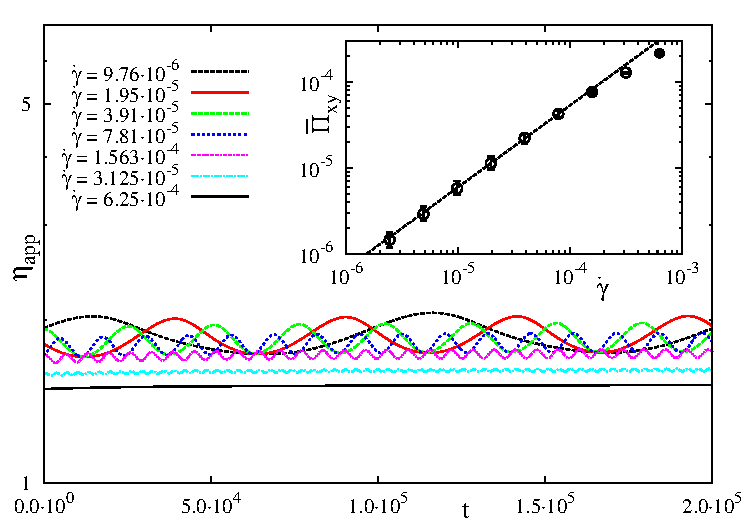
\includegraphics[width=0.495\textwidth]{stress_bp2.pdf}
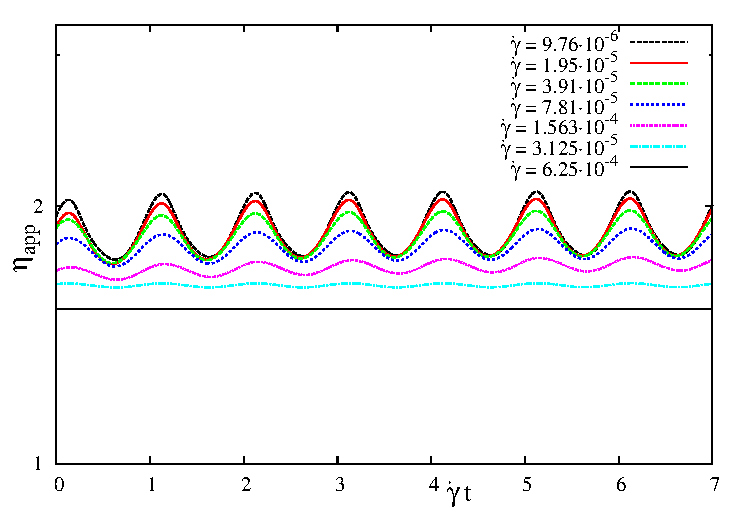
\includegraphics[width=0.495\textwidth]{stress_vs_strain_bp2.pdf}
\caption{Apparent viscosity $\eta_{app}=\Pi_{xy}/\eta\,\gd$ of BPII versus time (top) and strain (bottom). 
For clarity the individual curves have been shifted along the time and strain axis. 
The inset shows the flow curve $\bar{\Pi}_{xy}(\gd)$ and two different regimes of flow: 
regular periodic breakup and reconnecting of the disclination lines (BPII-1, open circles) 
and break up of the network into a travelling helical wave (BPII-2, solid circle).}
The error bars indicate the maximum and minimum stresses that occur during one cycle.
\label{bp2-rheo}
\end{figure}

We start our discussion with BPII as its flow behaviour turns out to be somewhat simpler 
than that of BPI. BPII has simple cubic symmetry and the disclination lines intersect and form a characteristic network of nodes.
Ahead of the more detailed discussion we provide first a general overview of the flow behaviour at all applied shear rates.
Fig. \ref{bp2-rheo} shows the apparent viscosity, which is defined as the 
deviatoric stress normalised to the isotropic background viscosity: 
$\eta_{app}=\Pi_{xy}/\eta\,\gd$.
A numerical value of $\eta_{app}=1$ corresponds to total shear thinning without 
any additional contribution from the liquid crystal.
The top picture shows the data over time, whereas the graph at the bottom gives 
the same data versus accumulated strain.
For all but the highest flow rates $\eta_{app}$ oscillates sinusoidally, which
is because of the periodic breakup and reconnecting of the network in shear flow. We refer to this regime as BPII-1.

The inset shows a flow curve, defined as time averages of 
the deviatoric stress tensor $\bar{\Pi}_{xy}$ as a function of shear rate $\gd$.
For all but the largest shear rates a power law fit $\bar{\Pi}_{xy}=a \gd^b$ with 
$a=0.35, b=0.95$ describes the data to a very good approximation. 
Hence, the degree of shear-thinning is remarkably small, but may depend
on the exact direction in which the strain is applied, an aspect that we     
leave for future work.

For shear rates $4.68\e{-4}\lesssim\gd\lesssim6.25\e{-4}$ the network of disclination lines
breaks up and oscillations in the stress signal are absent.
In this regime of shear rates, to which we refer as BPII-2, the 
blue phase dissolves into a simple cholesteric liquid 
crystal. The helical axis is oriented in vorticity direction and 
the mode of flow is a travelling helical wave.

At shear rates $7.81\e{-4}\lesssim\gd9.37\e{-4}$ the helix changes orientation.
The helical axis is now oriented along the gradient direction with
the liquid crystal flowing in 'nematic planes'. For even higher shear rates
the system undergoes a transition to a flow-aligned nematic state.

In the next paragraph we will investigate some of these aspects in more detail 
by looking at the kinetics of the disclination network.

\subsubsection{Regime BPII-1: low and intermediate shear rates}

Fig. \ref{bp2-med} shows the disclination network in shear flow as
it undergoes an affine transformation. The disclination lines break up and 
reconnect further downstream forming a periodically recurring pattern with 
recurrence time $\tau_F=1/\gd$ in flow direction.

\begin{figure}[htpb]
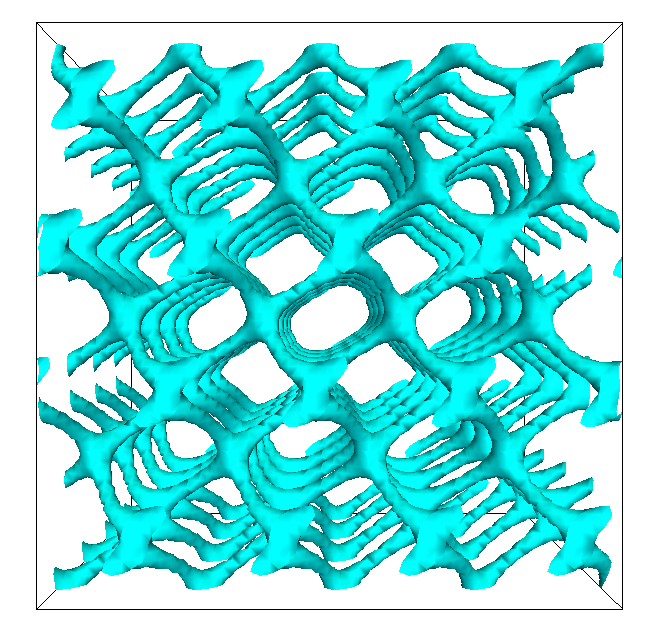
\includegraphics[width=0.41\textwidth]{disc-160k_run902.png}
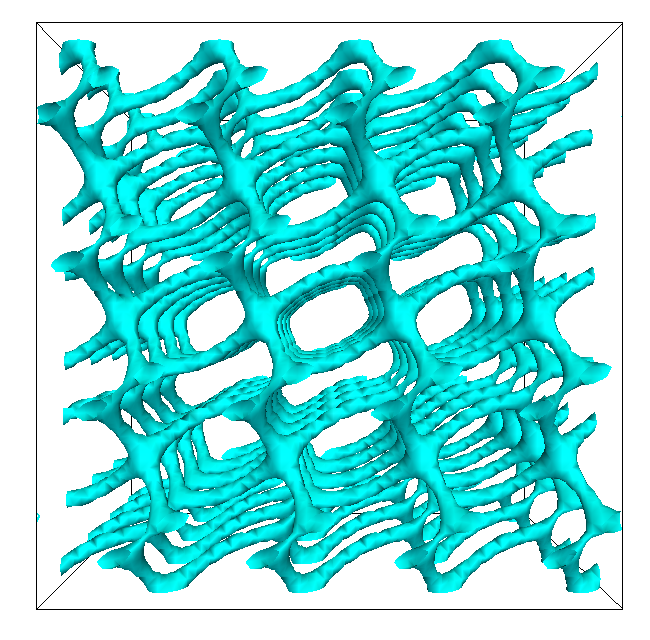
\includegraphics[width=0.41\textwidth]{disc-164k_run902.png}
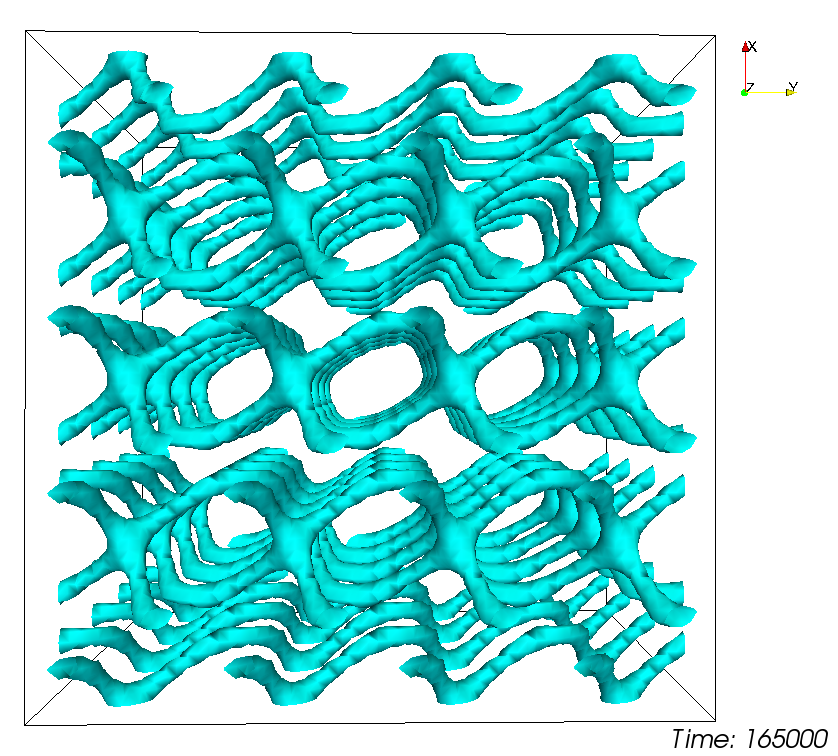
\includegraphics[width=0.41\textwidth]{disc-165k_run902.png}
\caption{Disclination network of BPII in shear flow: 
The pictures show a typical sequence of snapshots in the steady state 
at $\gd=1.56\e{-4}$ and time steps $t=1.60, 1.64,1.65\e{5}$. The velocity 
gradient is oriented along the vertical direction, whereas the 
horizontal direction is the flow direction. Lees-Edwards boundary 
conditions have been imposed in such a way that network moves to the 
right in the upper half and to the left in the lower half of the picture.}
\label{bp2-med}
\end{figure}

\begin{figure*}[htpb]
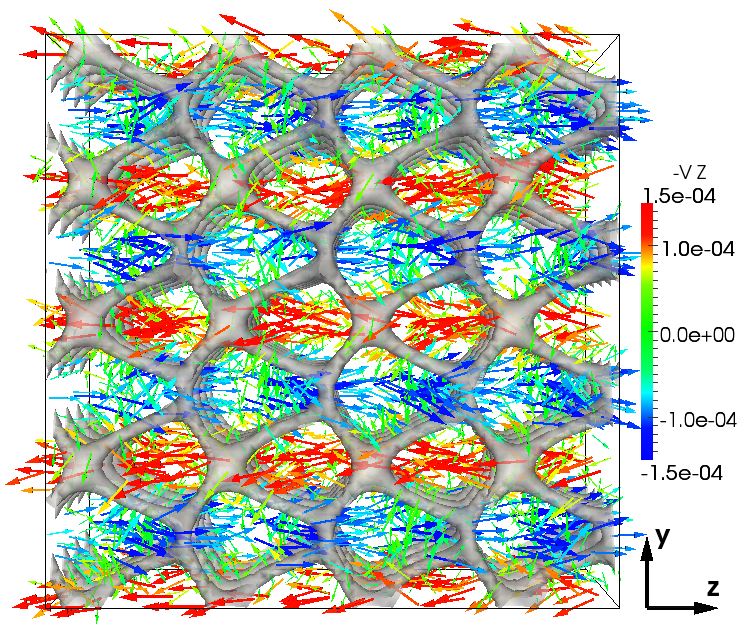
\includegraphics[width=0.495\textwidth]{v_yz-v_z-160k_run902.png}
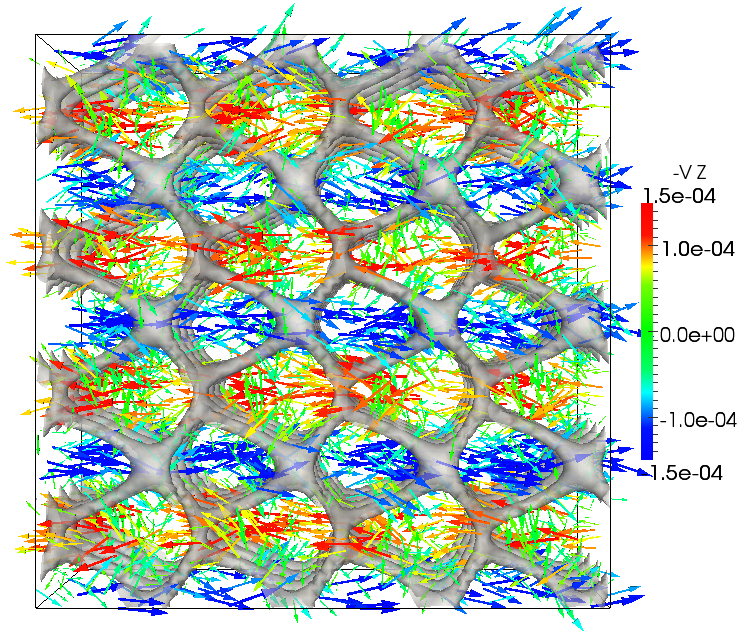
\includegraphics[width=0.495\textwidth]{v_yz-v_z-160k_run903.png}
\caption{Velocity patterns and disclination network in BPII for positive (left) and negative (right) helicity of the 
underlying cholesteric helix: The pictures show velocity vectors $(0,v_y,v_z)$.
The view is in x-direction. This means the velocity ${\mathbf v}$ 
has been projected onto a plane perpendicular to the flow direction. 
The vertical and horizontal direction are the gradient and vorticity direction, respectively.
The colour code gives the magnitude and sign of the component in vorticity direction.
The snapshot shows a typical frame during a periodically recurring sequence.
The network on the left with positive helicity travels rightwards, whereas the one one the right
moves leftwards. The recurrence period in vorticity direction is six times longer than the time it takes the network to reconnect in flow direction.}
\label{bp2-velo}
\end{figure*}

The general appearance of the flowing network is apart from the affine transformation 
very close to that of the quiescent blue phase at equilibrium. It is the same for 
all shear rates in regime BPII-1 and a first explanation why shear-thinning is so weak.

Interestingly, while being displaced with the flow the entire network moves 
in the vorticity direction.  A similar behaviour has been recently 
observed for blue phases in shear flow in 
confined geometries ~\cite{Henrich:2012b}.
In contrast to the stick-slip motion that has been reported there the movement is 
steady. It occurs in such a manner that the positions of breakup and reconnection 
of the network, visible in Fig. \ref{bp2-med}, are slightly offset and make the network 
travel along the z-direction.
The recurrence time in vorticity direction $\tau_V=6\tau_F$, 
i.e. it takes a displacement of six unit cells in flow directions 
until the network has moved one unit cell in vorticity direction.

Fig. \ref{bp2-velo} shows the disclination network between reconnecting 
and the next breakup with superimposed velocity vectors.
Shown are what we may call secondary velocity components, obtained by projecting the
velocity onto a plane perpendicular to the flow direction.
This gets rid of the dominating velocity component $v_x$ and 
allows to visualise the two much smaller components $v_y$ and $v_z$.
The magnitude of the secondary components is typically in the range of a 
few percent of the primary flow component.

Characteristic bands are visible in Fig. \ref{bp2-velo}, which are 
oriented along the vorticity direction. They are obscured by the
primary flow component if the above described projection procedure
is not applied.
When the helicity of the underlying cholesteric phase is changed from 
left-handed to right-handed, 
the pattern becomes a mirror image of the former one. The sign of 
$v_z$ changes and the sense of motion is inverted.
Further quantitative evidence for a direct link between the sense of motion 
and the helicity can be gained by time-averaging over individual cycles.
Tab. \ref{tab1} gives minima, maxima, averages and standard deviations 
of the velocity components.
All values for the two runs with inverted helicity are identical apart 
from a change of sign in the z-components.
There is only a slight imbalance between the maximum and minimum velocities 
in z-direction, suggesting that the movement of the network in vorticity 
direction is permeative. Note that this imbalance is retained under inversion of
helicity.

\subsubsection{Regime BPII-2: high shear rates}

If the flow rate exceeds a certain critical value BPII does not undergo the 
affine transformation  above and adopts another mode of flow. 
Fig. \ref{bp2-high} shows a sequence of cuts through the director 
field at high shear rate. The entire blue phase network has broken up 
into a simple cholesteric helix and flows as a travelling 
helical wave with the helical axis oriented along the vorticity direction.
The state is translationally invariant in flow and gradient direction.
and is the preferred mode of flow of a cholesteric 
liquid crystal in vorticity mode at low Ericksen numbers, i.e. below 
the uncoiling transition to a nematic, flow-aligned state at even 
higher shear rates ~\cite{Rey:1996a, Rey:1996b}.

In our scenario the break-up occurs for shear rates $\gd\simeq 4.68\e{-4}$, which
corresponds to Ericksen numbers of ${\it Er}\simeq4$, based on our
parameters for BPII ($K=0.02, \eta=0.666$, Tab. \ref{tab1} and $p_0/2=16$).

\begin{figure}[htpb]
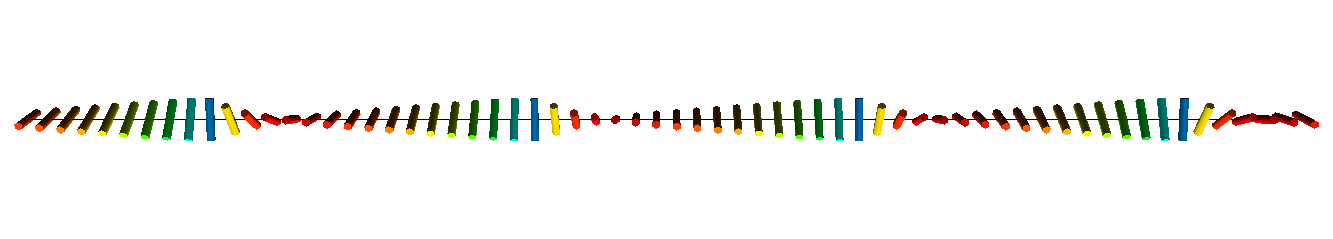
\includegraphics[width=0.495\textwidth]{dir+y-250k_run949.png}
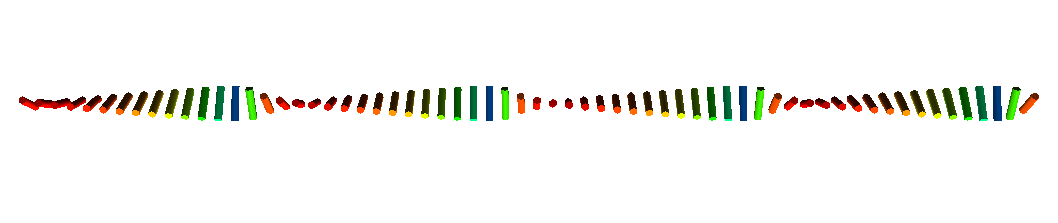
\includegraphics[width=0.495\textwidth]{dir+y-253k_run949.png}
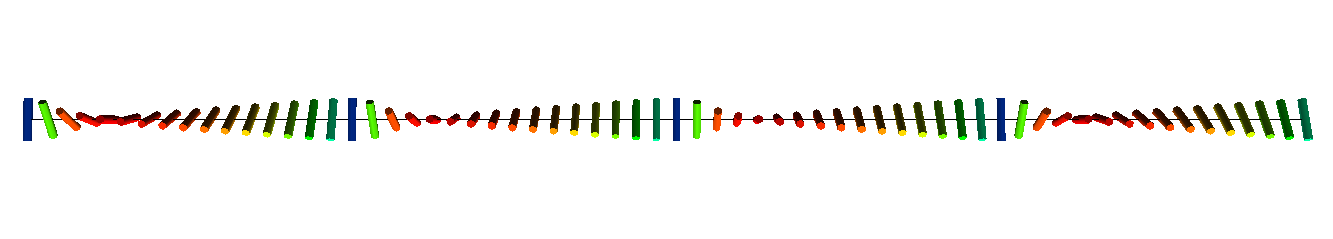
\includegraphics[width=0.495\textwidth]{dir+y-255k_run949.png}
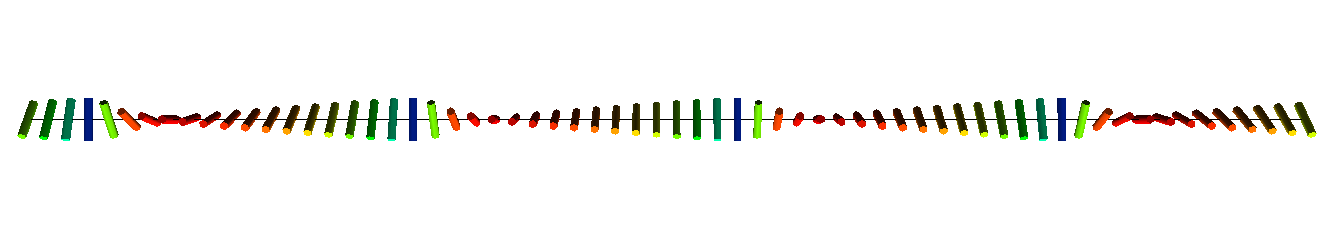
\includegraphics[width=0.495\textwidth]{dir+y-257k_run949.png}
\caption{Director field of BPII at high shear rate: The images show snapshots at time steps 
$t=2.50, 2.53,2.55, 2.57\e{5}$ (from top to bottom) with flow into/out of the page. 
The configuration is a helical wave that travels along the direction of vorticity.
It is translationally invariant in gradient and flow direction.}
\label{bp2-high}
\end{figure}

We observe another configuration between the travelling helical wave and the 
flow-aligned nematic state at shear rates $7.81\e{-4}\lesssim\gd\lesssim9.37\e{-4}$, 
which has so far not been reported to our knowledge \com{CHECK}.
We will address this in section \ref{cholflow}.

\subsection{Blue Phase I}

BPI has body-centered symmetry and unlike BPII. The disclination lines
 are well separated and do not intersect.
We believe that this topological difference is responsible for most of
the differences between BPI and BPII regarding their rheological response. 
We present again key aspects in an overview before we 
address some features in more detail. 

Fig. \ref{bp1-rheo} shows the apparent viscosity $\eta_{app}$ versus time and 
strain for the same shear rates as in Fig. \ref{bp2-rheo}.
For shear rates $9.37\e{-4}\lesssim\gd\lesssim1.25\e{-3}$ we observe the same cholesteric 
configuration with the helical axis along the gradient direction as for BPII (see
section \ref{cholflow}).
 
In regime BPI-3 $6.25\e{-4}\lesssim\gd\lesssim7.81\e{-4}$ a breakup of 
the blue phase disclination network occurs. This is about the same critical shear rate 
where we observe the transition to BPII-2. However, for BPI the configuration is not
a travelling helical wave, but rather a quasi two-dimensional state consisting of
double-twist rolls.

At shear rates $3.91\e{-5}\lesssim\gd\lesssim4.68\e{-4}$ we find flow with 
periodically recurring conformations. We refer to this regime as BPI-2. 
The oscillations in the 
deviatoric stress that are not sinusoidal, but show an increasingly complex
pattern up to the breakup point.
For even lower shear rates $\gd\lesssim3.91\e{-5}$ in regime BPI-1 
these oscillations become very erratic and unstable. 
There is no regular recurrence and 
after a few cycles the stress pattern is completely irregular.
Finally, the system ends up in an amorphous configuration.
Shear-thinning is slightly stronger than in BPII.
The average shear stress during one cycle can be fitted reasonably 
well by a power law $\bar{\Pi}_{xy}=a \gd^b$ with $a=0.019, b=0.63$.

\begin{figure}[htpb]
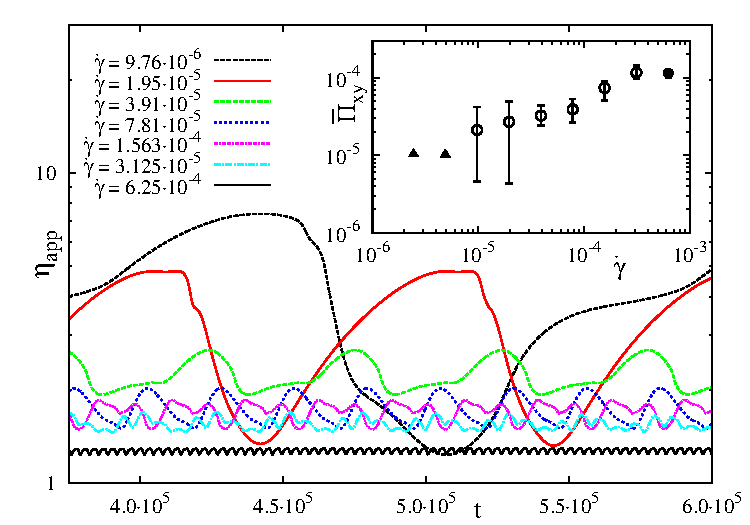
\includegraphics[width=0.495\textwidth]{stress_bp1.pdf}
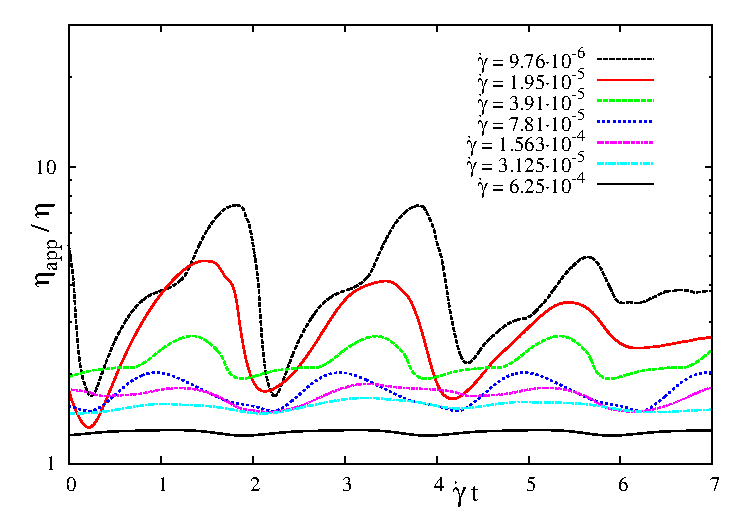
\includegraphics[width=0.495\textwidth]{stress_vs_strain_bp1.pdf}
\caption{Apparent viscosity $\eta_{app}=\Pi_{xy}/\dot{\gamma}$ of BPI versus time (top) 
and strain (bottom). The inset shows the flow curve $\bar{\Pi}_{xy}(\gd)$. 
Depending on the configuration in steady shear flow three different regimes 
can be identified: amorphous BP network with yield stress (BPI-1, triangles), 
steady flow with recurring patterns (BPI-2, open circles) and 
breakup of the disclination network (BPI-3, solid circle). 
The error bars represent the minimum and maximum shear stress 
during one cycle. For clarity the individual curves have been shifted along
the time and strain axis.}
\label{bp1-rheo}
\end{figure}

In order to gain a better understanding of the complex oscillatory behaviour in regime BPI-2 
we performed a Fourier analysis of the deviatoric stress $\Pi_{xy}$ according to Eq. \ref{spectrum}. 
The spectrum is shown in Fig. \ref{bp1-spectrum}. 

There are two aspects which are worth mentioning. First, we observe a strong contribution of 
the fundamental mode for the lowest two shear rates and a relatively small contribution of higher harmonics. 
However, at $\gd=1.563\e{-4}$ and $3.125\e{-4}$ the relative contribution of higher harmonics is 
significantly larger. 
More surprisingly the frequency of the fundamental mode is the same 
for all three shear rates $\gd=7.81\e{-5}, 1.563\e{-4}$ and $3.125\e{-4}$. This is 
in contrast to what is observed at lower flow rates. By doubling the flow rate from 
$\gd=3.91\e{-5}$ to $\gd=7.81\e{-5}$ the peak position in the spectrum 
moves to the double frequency. This means that the fundamental mode at flowrate $\gd=7.81\e{-5}$ 
coincides with the the first harmonic at $\gd=3.91\e{-5}$, the first harmonic with the third and so on,
which is the expected behaviour. At higher shear rates in regime BPI-3 this 'lock-in' of 
flow modes disappears again.  
 
Interestingly the lock-in has only a minor effect on the flow velocities themselves.
The average velocities in Tab. \ref{tab1} reveal that only the magnitude of some of the secondary 
flow components $v_y$ and $v_z$ appears to be relatively small compared to the primary component $v_x$. 
The latter is directly linked to the imposed shear rate. 

\begin{figure}[htpb]
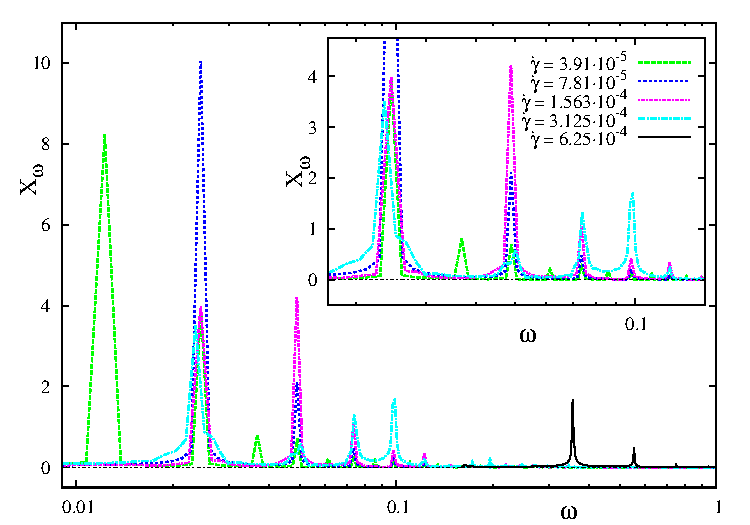
\includegraphics[width=0.495\textwidth]{spectrum_bp1.pdf}
\caption{Fourier analysis of the deviatoric stress $\Pi_{xy}$ of BPI: The main picture shows 
spectral components and the 'lock-in' of flow modes, 
visible in the fixed peak position for certain flow rates.  
The inset shows the same data on an expanded scale. 
The frequency is given in radians.}
\label{bp1-spectrum}
\end{figure}

\subsubsection{Regime BPI-1: low shear rates}

\begin{figure}[htpb]
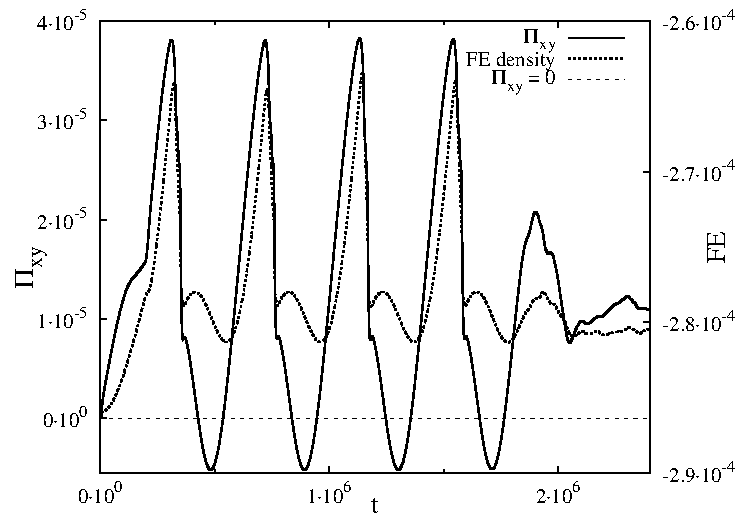
\includegraphics[width=0.495\textwidth]{stress_fe_yield_bp1.pdf}
\caption{Average deviatoric stress and free energy density of BPI at low shear rate: 
The negative branch in the stress is related to a local maximum and a following local 
minimum in average free energy density. This creates unstable conditions that lead 
to a dissolving regular network and an amorphous state which features a yield stress.}
\label{bp1-fe-yield}
\end{figure}

The rheological response of BPI at low shear rate $\gd<3.91\e{-5}$ 
is strikingly different from that of BPII and exhibits a
dynamic yield stress.
An explanation for this strange behaviour can be found by 
looking more closely at the average deviatoric stress and 
free energy density, as shown in Fig. \ref{bp1-fe-yield}.
When the quiescent and equilibrated BPI network begins to flow
the shear stress increases steeply and goes through a global maximum.
Shortly after it goes negative (the total shear stress is still
positive as the background viscosity has been subtracted) and then positive
again, forming a complete cycle. 
This cycle is repeated for a couple of times before 
any regular pattern disappears and the amorphous configuration 
emerges.

\begin{figure*}[htpb]
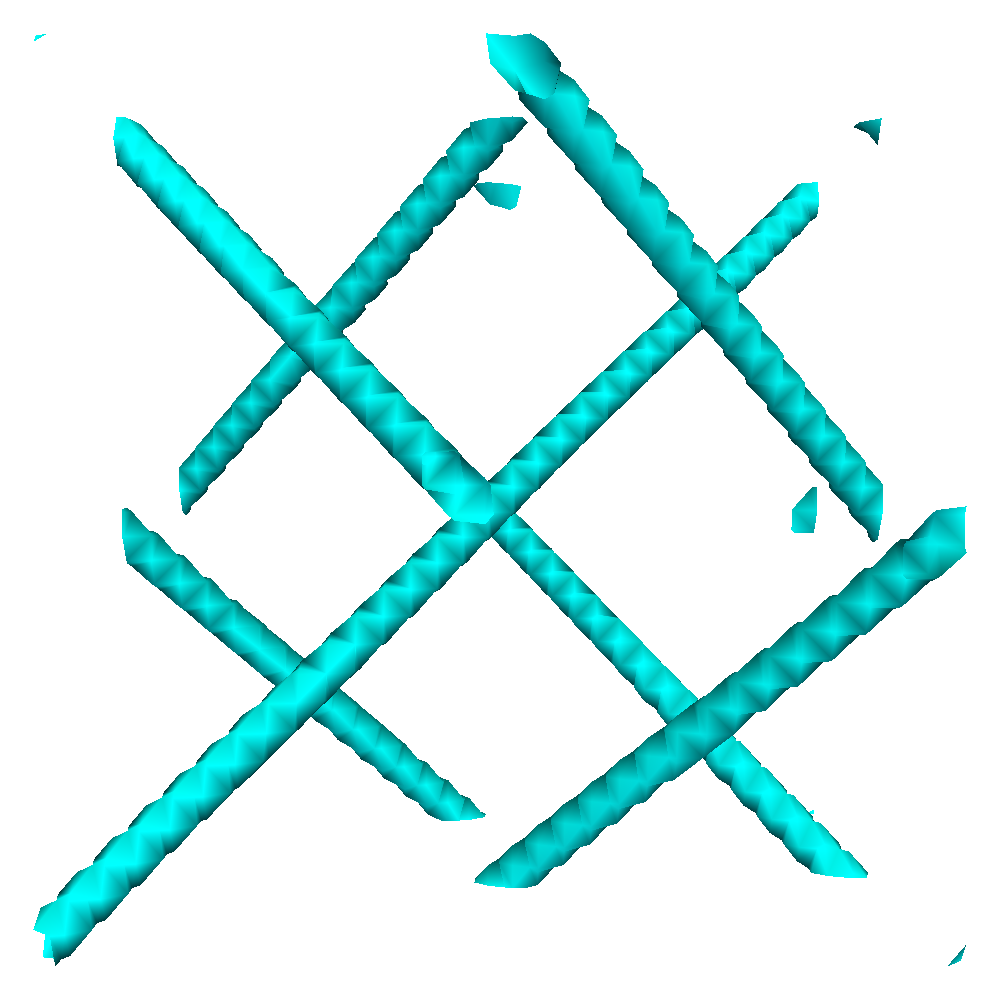
\includegraphics[width=0.245\textwidth]{disc-xy-10k_run1115.png}
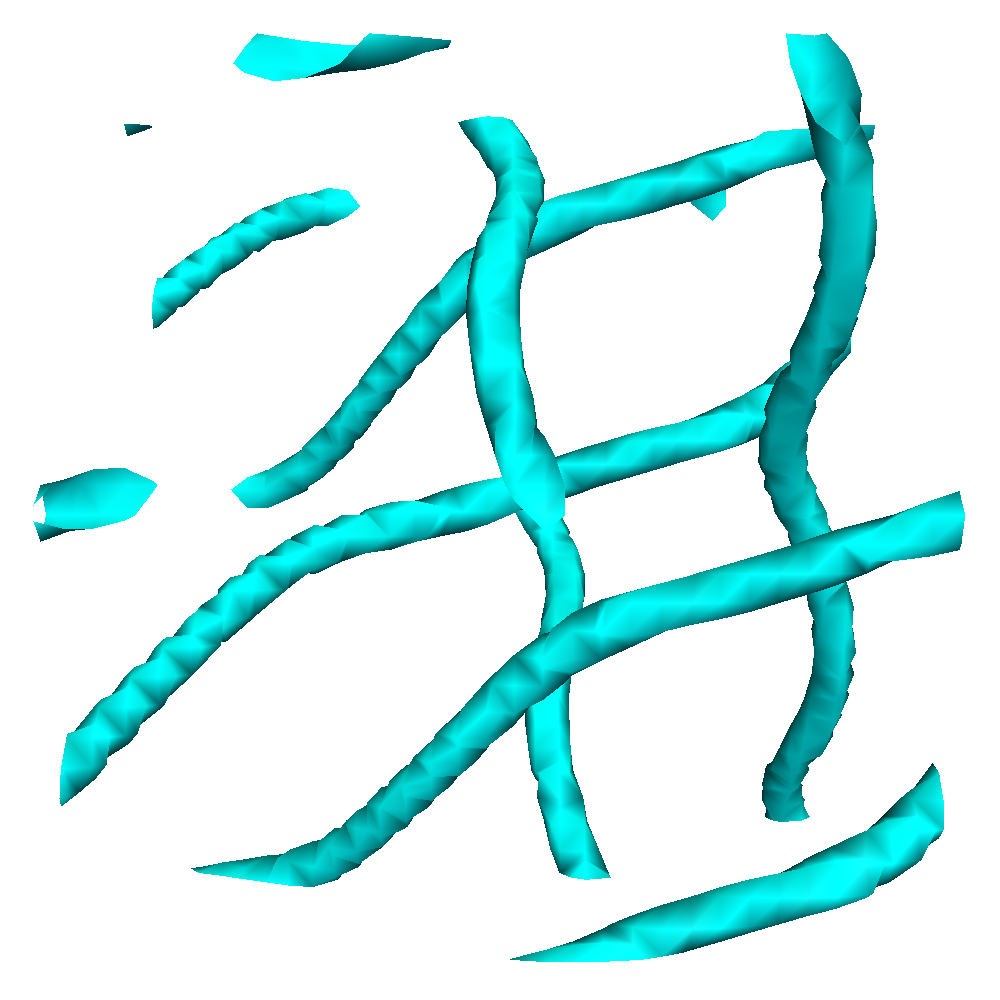
\includegraphics[width=0.245\textwidth]{disc-xy-180k_run1115.png}
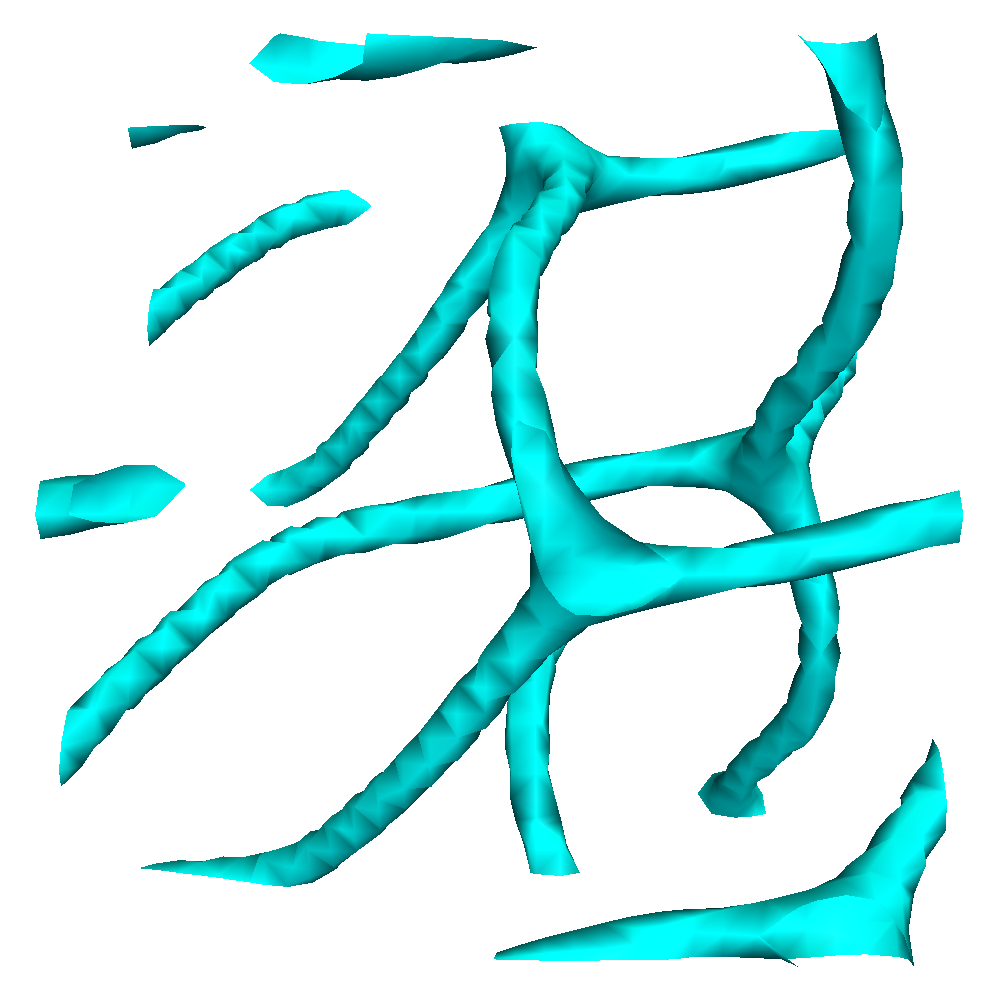
\includegraphics[width=0.245\textwidth]{disc-xy-200k_run1115.png}
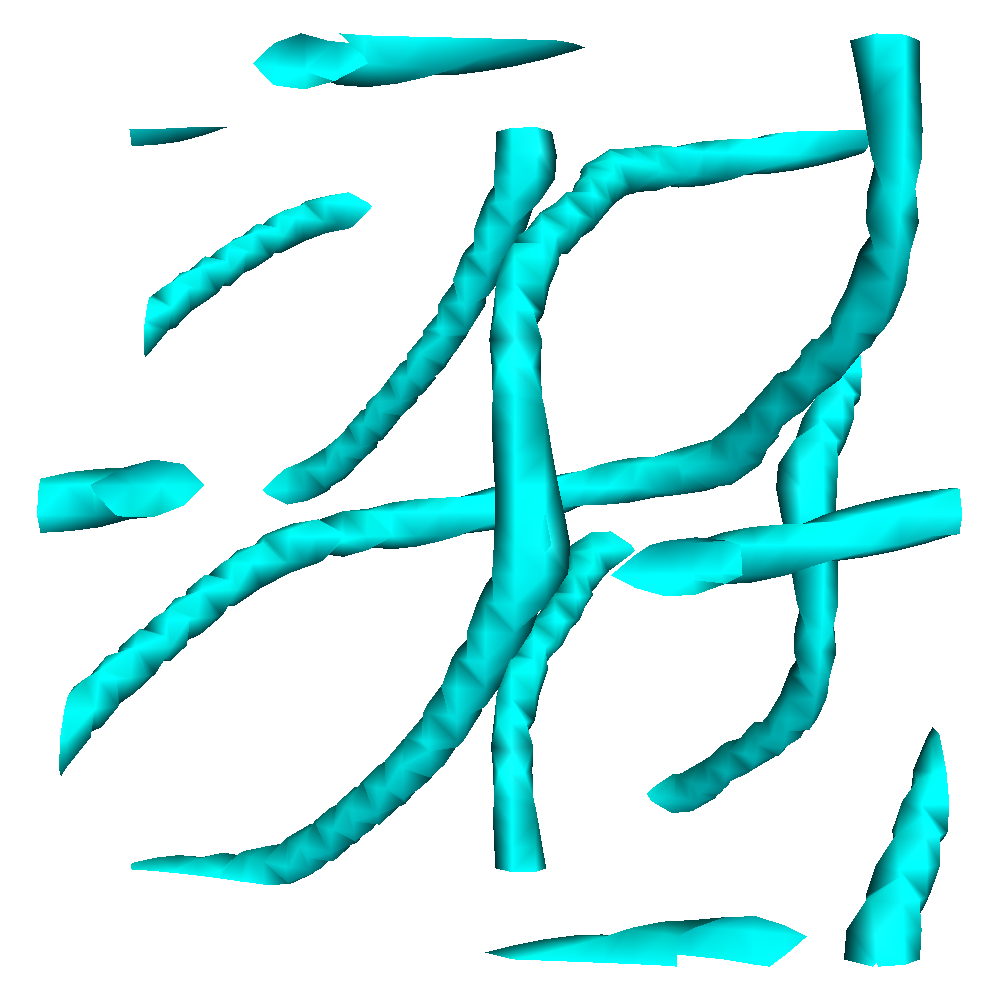
\includegraphics[width=0.245\textwidth]{disc-xy-210k_run1115.png}\\
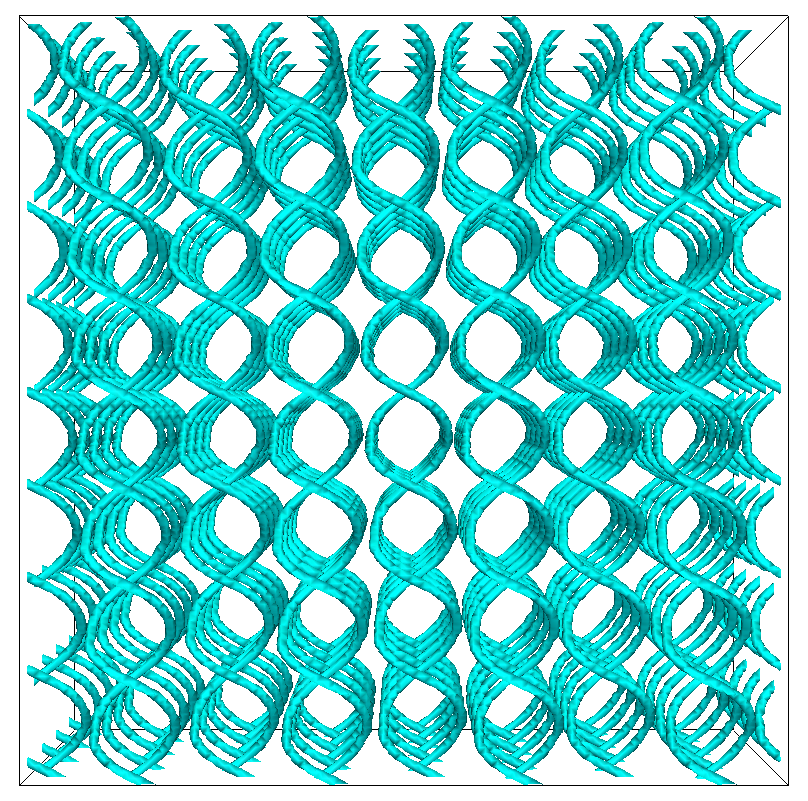
\includegraphics[width=0.245\textwidth]{disc-xy-400k_run1115.png}
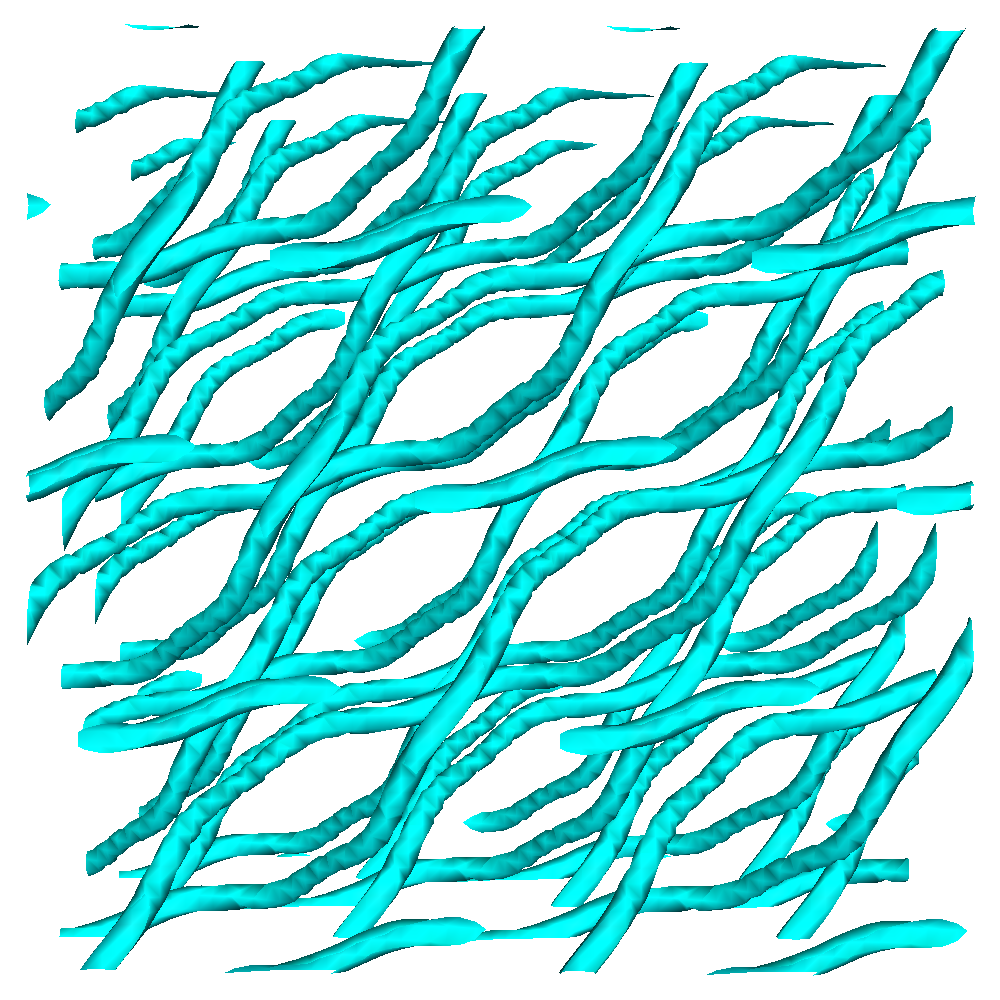
\includegraphics[width=0.245\textwidth]{disc-xy-700k_run1115.png}
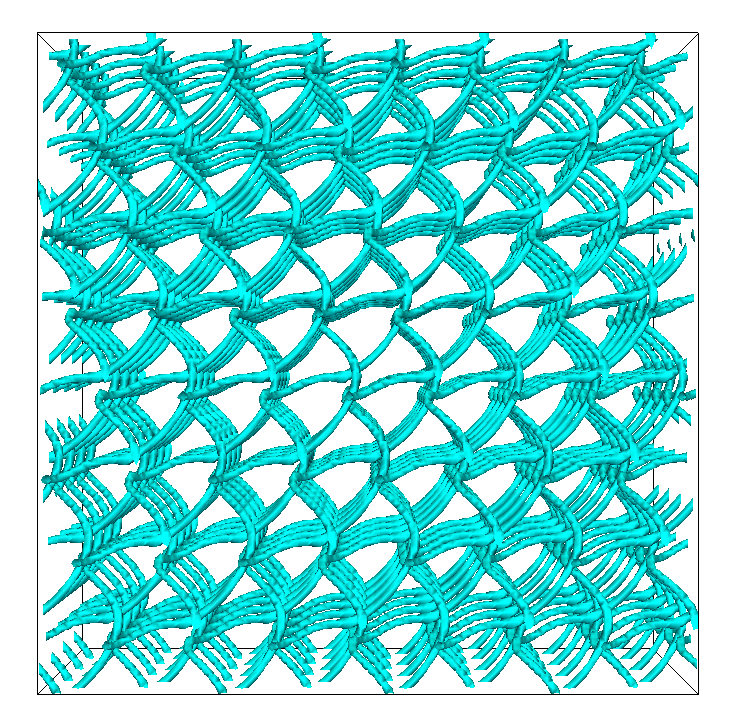
\includegraphics[width=0.245\textwidth]{disc-xy-750k_run1115.png}
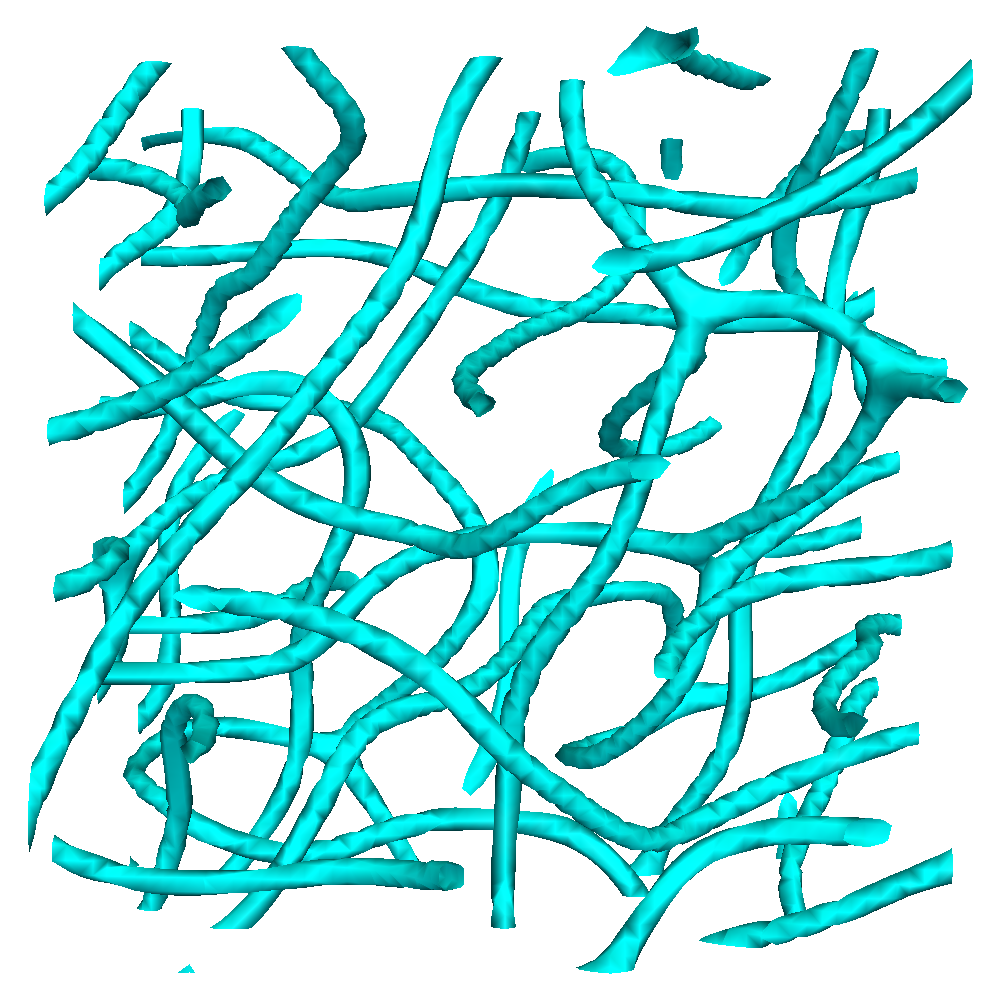
\includegraphics[width=0.245\textwidth]{disc-xy-2200k_run1115.png}
\caption{Snapshots of BPI disclination network at $\dot{\gamma}=4.88\e{-6}$: 
Depicted is the transition from the quiescent state to flow-induced, intertwined 
helices that undergo a recurring affine transformation. The top row
shows a section of one unit cell for early times 
$t=1\e{4}, 1.8\e{5}, 2.0\e{5}$ and $2.1\e{5}$. The bottom 
pictures on the far left, centre left and centre right 
show the situation at later time steps $t=4.0, 7.0$ and $7.5\e{5}$,
which the system passes for several cycles before it ends up in
an amorphous state (bottom row far right at time step $t=2.2\e{6}$).}
\label{bp1-low}
\end{figure*}

The negative branch in the deviatoric stress is connected
to a local maximum followed by a local minimum in the average free energy.
Hence, the region of negative stress can be 
regarded as a phase during which elastic forces exert a 
'pull' on the network while it tries to reach a more 
favourable configuration. However, the low flow rate
causes this unstable intermediate state to be exposed to these
elastic forces for a relatively long time, long enough to 
create small distortions which finally break the symmetry of the
flow-induced configuration.

\begin{figure}[htpb]
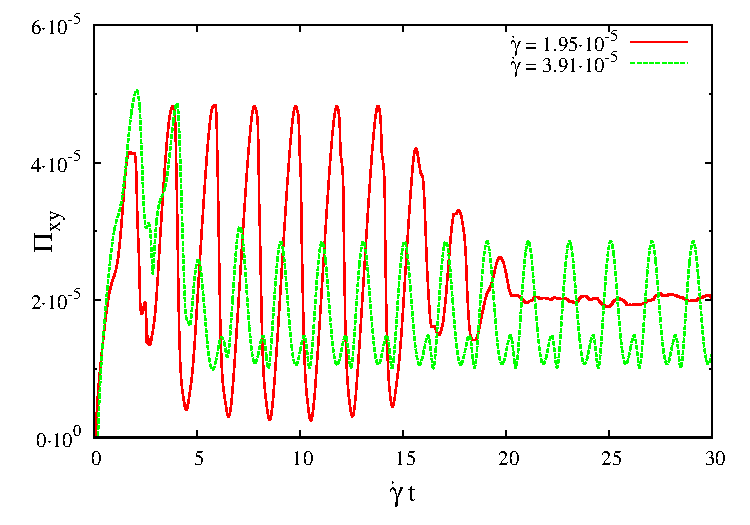
\includegraphics[width=0.495\textwidth]{stress_bp1-1_bp1-2.pdf}
\caption{Deviatoric stress $\Pi_{xy}$ versus strain at the transition between regime
BPI-1 and BPI-2. The shear rates are $\gd=1.95\e{-5}$ (red solid) 
and $\gd=3.91\e{-5}$ (green dashed). Compared to lower shear rates in BPI-1 
where the stress goes negative (Fig. \ref{bp1-fe-yield}) the stress is 
throughout positive, but exhibits very large fluctuations during one cycle, 
which are absent in regime BPI-2 at higher shear rates.}
\label{bp1-1_bp1-2}
\end{figure}

We want to explain these differences on the basis of a typical 
appearance of BPI at low flow rate, which is depicted in Fig. \ref{bp1-low}.
Three different stages can be distinguished. 
With the onset of shearing the disclination lines 
in BPI get more and more squeezed together which is incommensurable with 
the defect topology of this blue phase. 
Consequently, the network adopts a flow-induced conformation which consists 
of intertwined helices that stretch during the affine transformation.
This helical conformation that emerges already at strains $\gamma\simeq1$ 
is shown in Fig. \ref{bp1-low} (top row).
At a particular point in the cycle a non-helical configuration is
observed (bottom left) before the network quickly returns
to its helical state. There is no perceivable movement of the 
network in vorticity direction at any stage of the cycle.

However, this mode of flow proves unstable as after a few cycles 
distortions appear which lead to further destabilisation.
Finally, the network loses any residual order and 
transforms into an amorphous state with almost constant
yield stress in the region of $\Pi_{xy}\simeq 1\e{-5}$ in LBU.

\subsubsection{Regime BPI-2: intermediate shear rates}

Adjacent to regime BPI-1 ($\gd<3.91\e{-5}$) and 
at slightly larger shear rates $3.91\e{-5}\le\gd< 6.25\e{-4}$
and Ericksen numbers $0.67\le{\it Er}<8$ 
lies another region where the network flows with periodically 
recurring conformations (Fig. \ref{bp1-rheo}). 
We refer to this region as BPI-2. The transition between BPI-1 and BPI-2 
is shown in Fig. \ref{bp1-1_bp1-2} by means of the deviatoric stress versus total strain. 
A qualitative difference between these two is the absence of 
large stress fluctuations that occur during one typical cycle in regime BPI-1.
Remember that for even lower $\gd$ the deviatoric stress becomes 
temporarily negative (Fig. \ref{bp1-fe-yield}), which 
caused destabilisation of the periodic network and led to the 
amorphous configuration in the steady state. Hence, an explanation 
for this phenomenon could be that in BPI-2 the network finds a 
kinetic path to bypass these large amplitude fluctuations that 
prevents the network from destabilising.

Fig. \ref{bp1-med} shows snapshots of the periodically recurring 
BPI in steady shear flow. Contrary to BPII-1 at these shear rates
, BPI-2 does not resemble the equilibrium configuration
undergoing an affine transformation. It features rather intricate, flow-induced 
conformations. Surprisingly this state is kinetically connected to the equilibrium 
state as when the shear flow is switched off the flow-induced configuration 
reverts to a perfect quiescent BPI unless it got stuck in a local free energy 
minimum. 

The recurrence period of conformations with visually similar appearance is 
less straightforward to determine. In the flow direction relation like
$\tau_F=n/\gd$ holds with $n=1,2,4$ for $\gd=3.91\e{-5},
7.81\e{-5},1.563\e{-4}$ for example. The analysis is complicated by the fact
that for $n>1$ thermodynamically equivalent, mirror-image 
conformations arise after shorter times. For instance at $\gd=7.81\e{-5}$
the conformations at times $t$ and $t+1/\gd$ are mirror-images, whereas
those at $t$ and $t+2/\gd$ coalesce in flow direction.

However, there is no definite recurrence period $\tau_V$ 
in the vorticity direction. The direction of the displacement
in other directions (i.e. both in gradient and vorticity direction) 
is not simply along coordinate directions. 
The magnitude of the displacement show no clear pattern, is non-integer 
and depends sensitively on the imposed shear rate,
suggesting BPI-2 constitutes an instance of 'rheochaos' [ref].

\begin{figure*}[htpb]
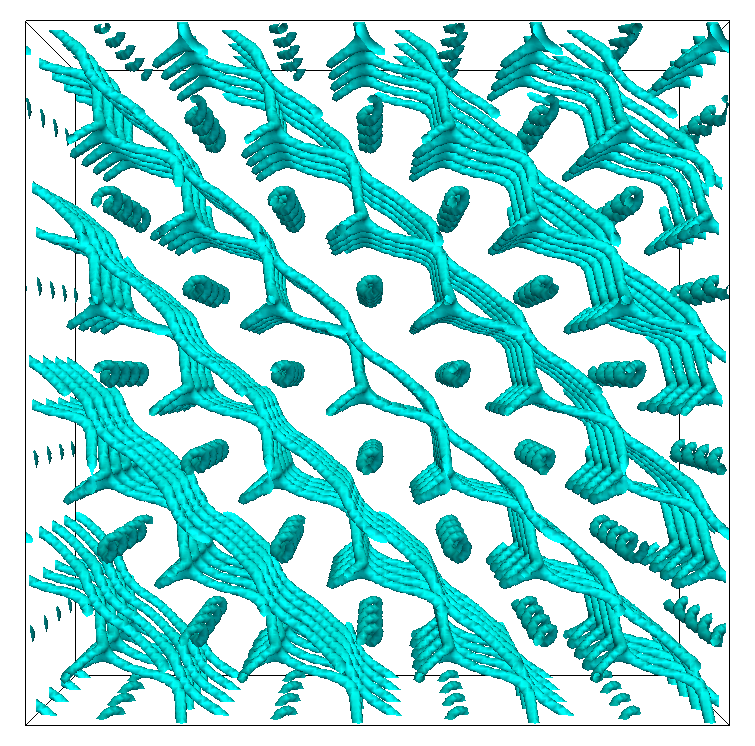
\includegraphics[width=0.32\textwidth]{disc-365k_run914.png}
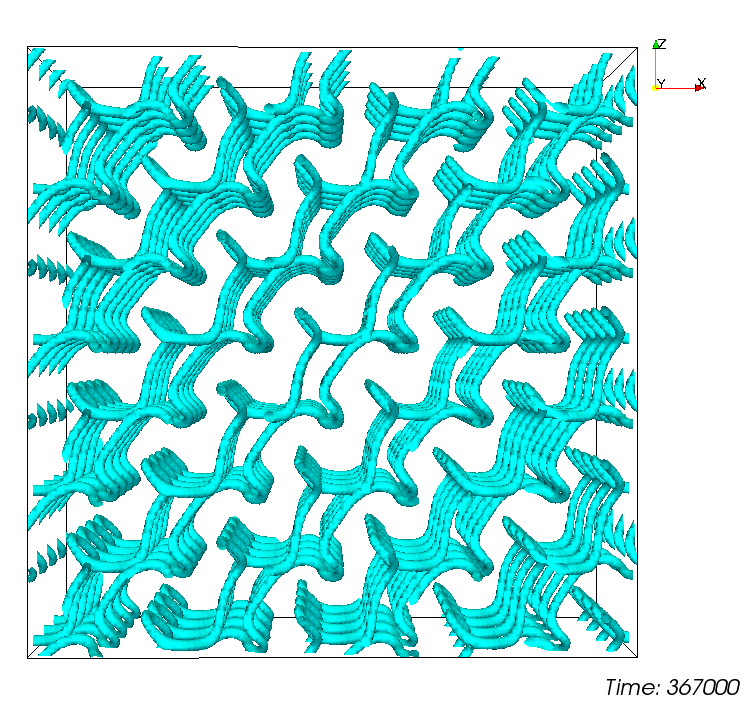
\includegraphics[width=0.32\textwidth]{disc-367k_run914.png}
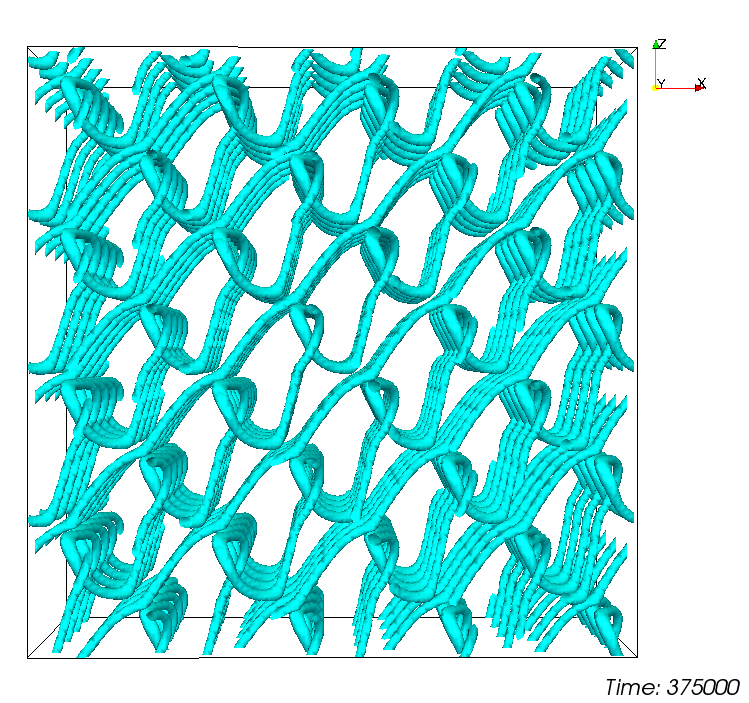
\includegraphics[width=0.32\textwidth]{disc-375k_run914.png}\\
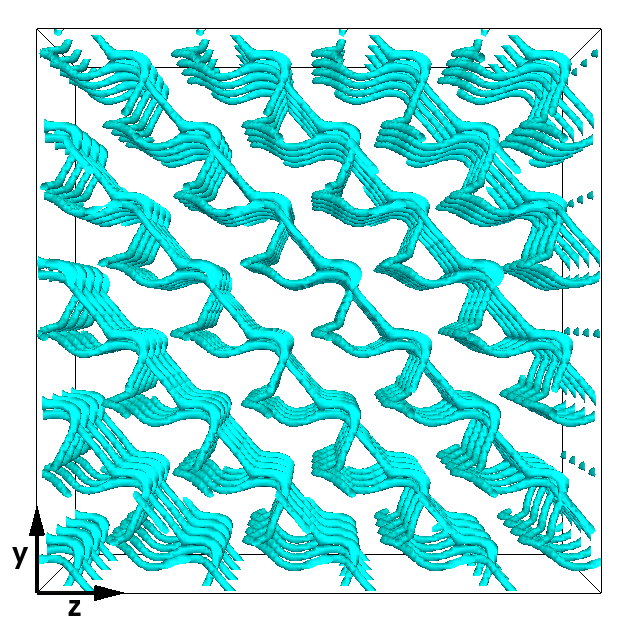
\includegraphics[width=0.32\textwidth]{disc-380k_run914.png}
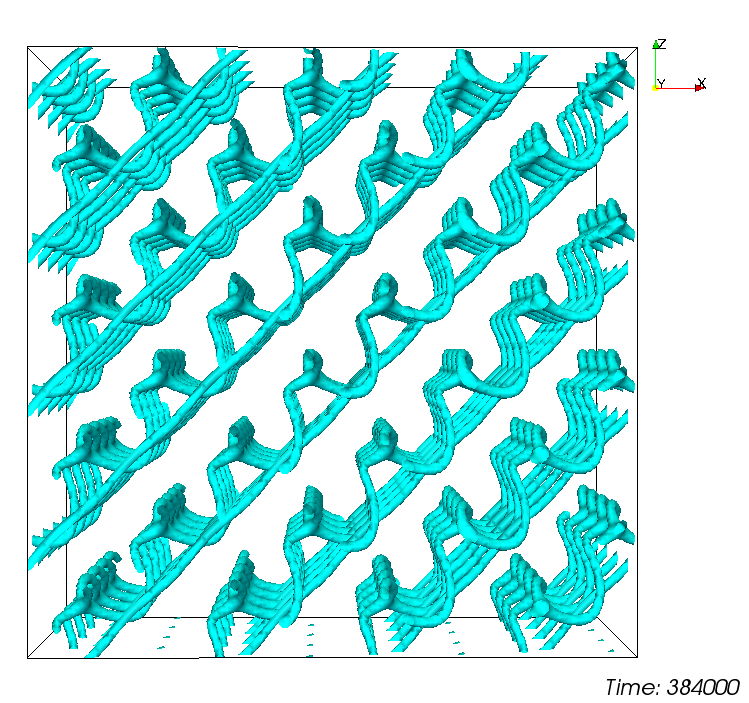
\includegraphics[width=0.32\textwidth]{disc-384k_run914.png}
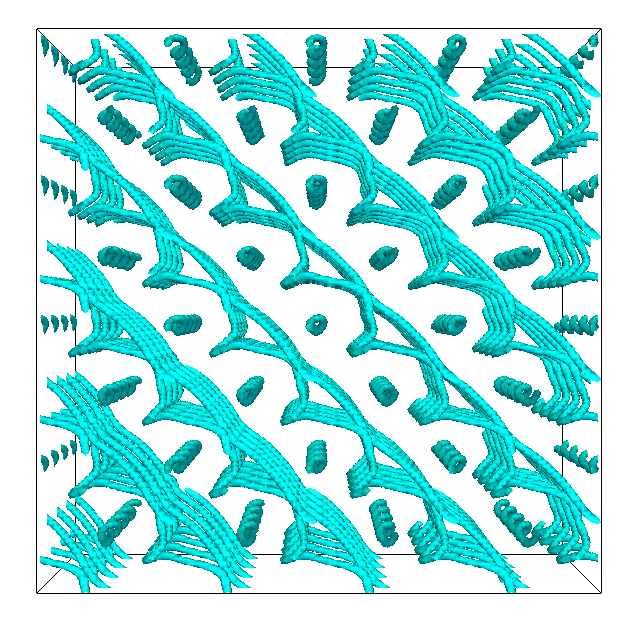
\includegraphics[width=0.32\textwidth]{disc-389k_run914.png}
\caption{Disclination network of BPI in regime BPI-2 (intermediate flow rates): 
The sequence shows a typical cycle of shear-induced transformations in the 
steady state at $\gd=1.56\e{-4}$ and time steps 
$t=3.65, 3.67,3.75,3.80,3.84,3.89\e{5}$ with the flow into/out of the page. 
During every cycle the network is displaced in gradient and vorticity direction, 
but the magnitude and direction of the offset appear to be chaotic and do not 
obey a simple rule.}
\label{bp1-med}
\end{figure*}

Fig. \ref{bp1-velo} depicts a snapshot of the secondary velocity 
components $v_y$ and $v_z$ for left- and right-handed cholesteric
helix. The emerging pattern is similar to that of BPII from 
Fig. \ref{bp2-velo}, but differs in that there is no
arrangement in bands. However, just as in case of BPII, both patterns
are mirror images and feature the highest velocities in the regions where 
the largest conformational changes take place. 

\begin{figure*}[htpb]
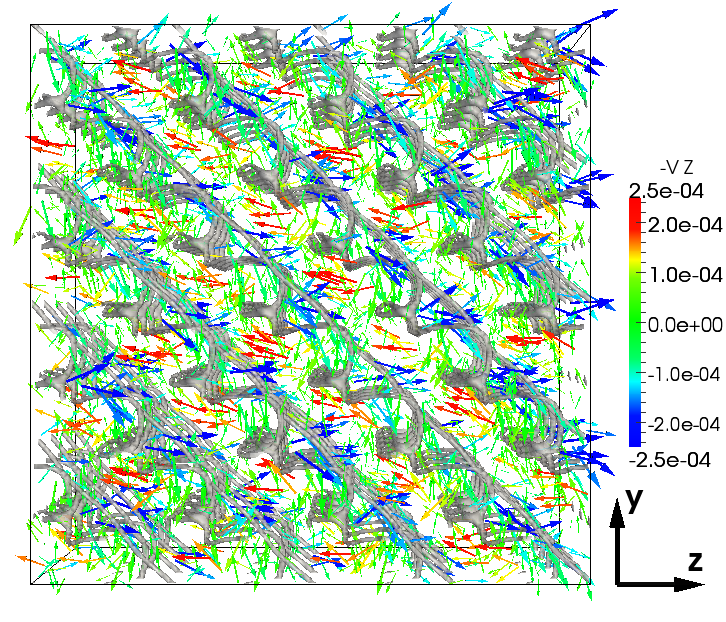
\includegraphics[width=0.495\textwidth]{v_yz-v_z-360k_run914.png}
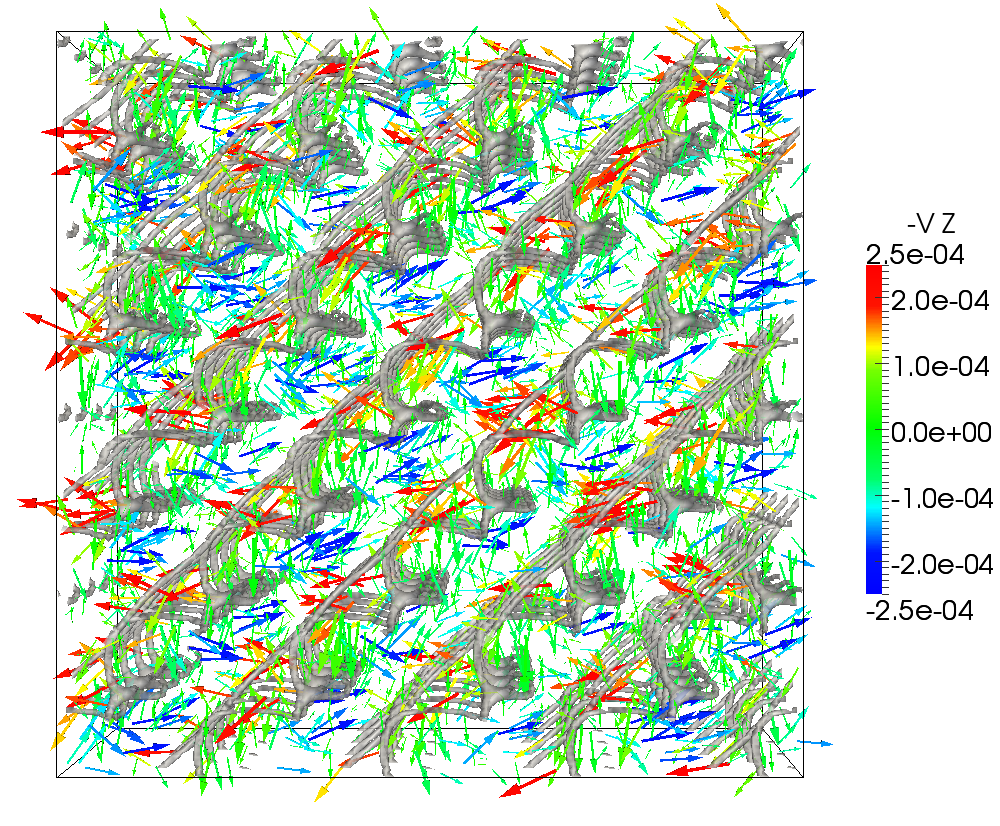
\includegraphics[width=0.495\textwidth]{v_yz-v_z-360k_run922.png}
\caption{Velocity patterns in BPI for positive (left) and negative (right) helicity: 
The pictures show a snapshot of the periodically recurring patterns in the 
secondary velocity components $(0,v_y,v_z)$, i.e. the component $v_x$ in flow direction 
has been projected out. The colour code gives the magnitude and sign 
of the z-component. The vertical and horizontal direction are the gradient and 
vorticity direction, respectively, with the flow into/out of the plane in the 
upper/lower half of the images.}
\label{bp1-velo}
\end{figure*}

The intricacy and periodic recurrence of the flow-induced conformations 
in BPI raises the question: how robust these results are with respect to 
system size? Although a pitch length of 64 LBU provides enough resolution 
for tracking the network in flow it is not clear whether $4^3=64$ unit cells 
in total are actually sufficient to avoid finite size effects.
Unfortunately the computational costs of larger simulations are still
prohibitive, given that large strains have to
be simulated in order to reach a steady state. Therefore we opted for a 
comparison with smaller runs.

Fig. \ref{bp1-2uc4uc} shows a comparison of the disclination network and 
deviatoric stress $\Pi_{xy}$ of to different runs, one consisting of 8 
unit cells and the other one with 64 unit cells.
Obviously there are large deviations in both the visual appearance of the 
network as well as in the time-dependence of the deviatoric stress.
In the smaller run with $2^3=8$ unit cells takes BPI also considerably 
to reach the 
steady state with its flow-induced recurring disclination network. 

These results indicate that we cannot know with certainty if the individual 
flow-induced conformations that we find for 64 unit cells are not affected 
by imposed periodicity. Nevertheless, the comparison suggests that 
the recurrence period and the complexity of the network in flow are  
generic features of BPI in this regime of flow.
 
\begin{figure}[htpb]
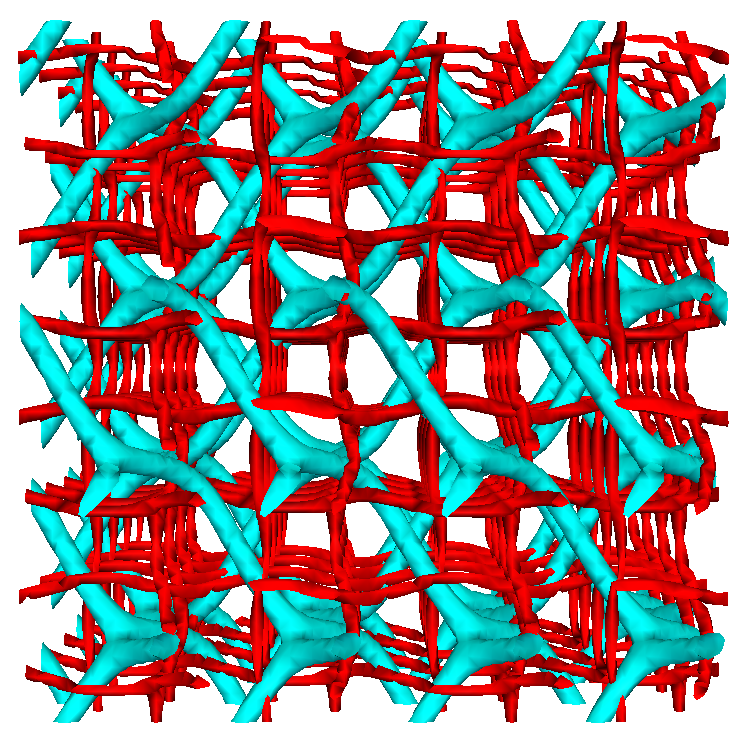
\includegraphics[width=0.43\textwidth]{disc+y-600k-run911_run1163.png}\\
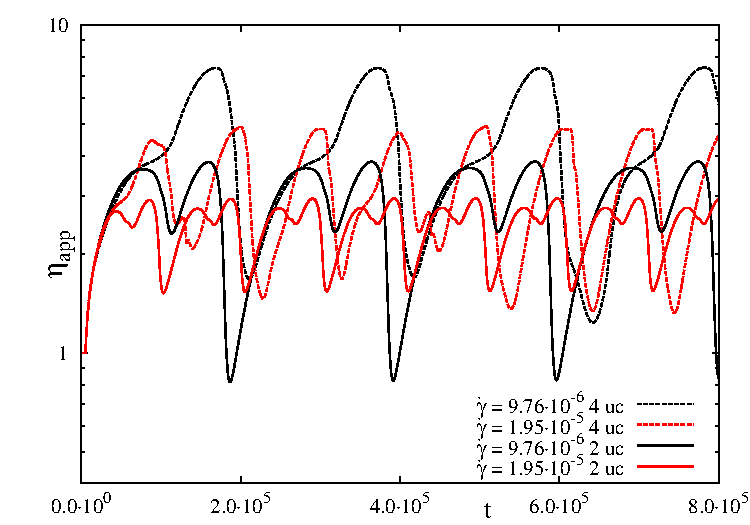
\includegraphics[width=0.495\textwidth]{stress_bp1_2uc_4uc.pdf}
\caption{Disclination network and deviatoric stress $\Pi_{xy}$ in BPI: 
The dark (red) network in top picture shows a snapshot of run that consists 
of $2^3=8$ unit cells, whereas the light (cyan) network displays the 
central section of 8 unit cells in a bigger run with $4^3=64$ unit cells altogether. 
The bottom picture shows the deviatoric stress over time. Interestingly, 
an intermediate sized run with $3^3=27$ unit cells led to results that 
were identical to the smaller run with 8 unit cells. The shear rate was $\gd=7.81\e{-5}$.
}
\label{bp1-2uc4uc}
\end{figure}

\subsubsection{Regime BPI-3: high shear rates}

\begin{figure}[htpb]
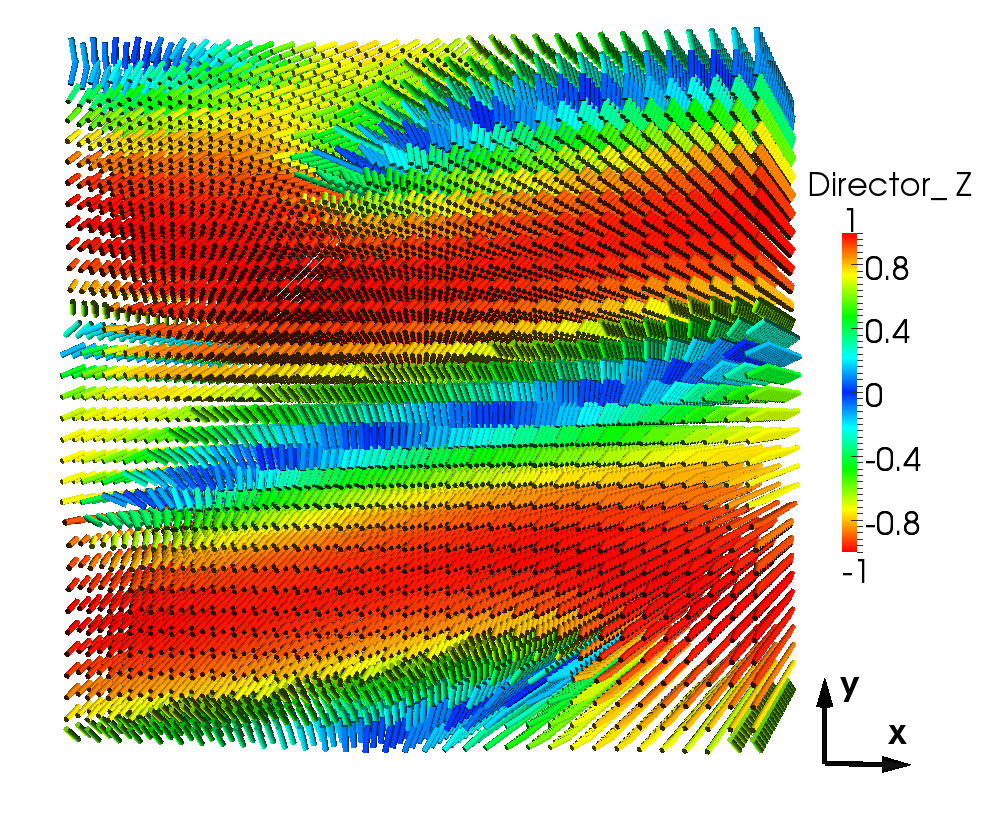
\includegraphics[width=0.45\textwidth]{dir3d-z-302k_run916.png}
\caption{Director field of BPI at high shear rate: The pictures show a region 
of $L_x\times L_y \times L_Z= 32^3$ lattice sites with the flow/gradient 
direction oriented along the horizontal/vertical axis. 
The colour code gives the magnitude of the z-component of the director field. 
The data is translationally invariant in vorticity direction.}
\label{bp1-high}
\end{figure}
 
At high flow rates $6.25\e{-4}\lesssim\gd\lesssim7.81\e{-4}$ 
we observe a break-up of the flow-induced 
disclination network of regime BPI-2. However, 
in contrast to BPII, where the configuration is a travelling helical 
wave (viz. Fig. \ref{bp2-high}), BPI prefers a quasi 
two-dimensional, translationally invariant state, which is shown in 
Fig. \ref{bp1-high}. The snapshots visualise the affine 
transformation of simple shear flow in the gradient-flow plane.
There are distinctive regions where the director field is 
predominantly oriented along the vorticity direction and 
other regions where it is oriented rather in flow-gradient plane. 
Occasionally while moving past each other these rolls resemble 
regions of local double twist.
Interestingly the critical Ericksen number for the break-up lies in 
about the same window as that of transition between BPII-1 and BPII-2. 

\subsection{Transition to cholesteric helix and flow-aligned nematic state}\label{cholflow}

At shear rates beyond the regimes BPI-3 and BPII-2 and below the transition to a 
flow-aligned nematic state we found another regime where 
both blue phases adopt the same configuration in steady shear flow, 
independent of their initial state.
The director field of this configuration is shown in Fig. \ref{cholflow}.
It consists of a simple cholesteric helix with the helical axis oriented 
along the gradient direction. The state is translational invariant in 
flow and vorticity direction and therefore also one-dimensional. 
However, in contrast to the travelling helical wave of BPII-2 the 
director field is now static and there is no tumbling motion. 
While flowing the director retains its relative orientation.
Consequently, the shear stress is lower than for
the 2D double-twist rolls of BPI-3 and the travelling helical wave
(Fig. \ref{bp2-rheo} and \ref{bp1-rheo}) as there is less dissipation.
 

\begin{figure}[htpb]
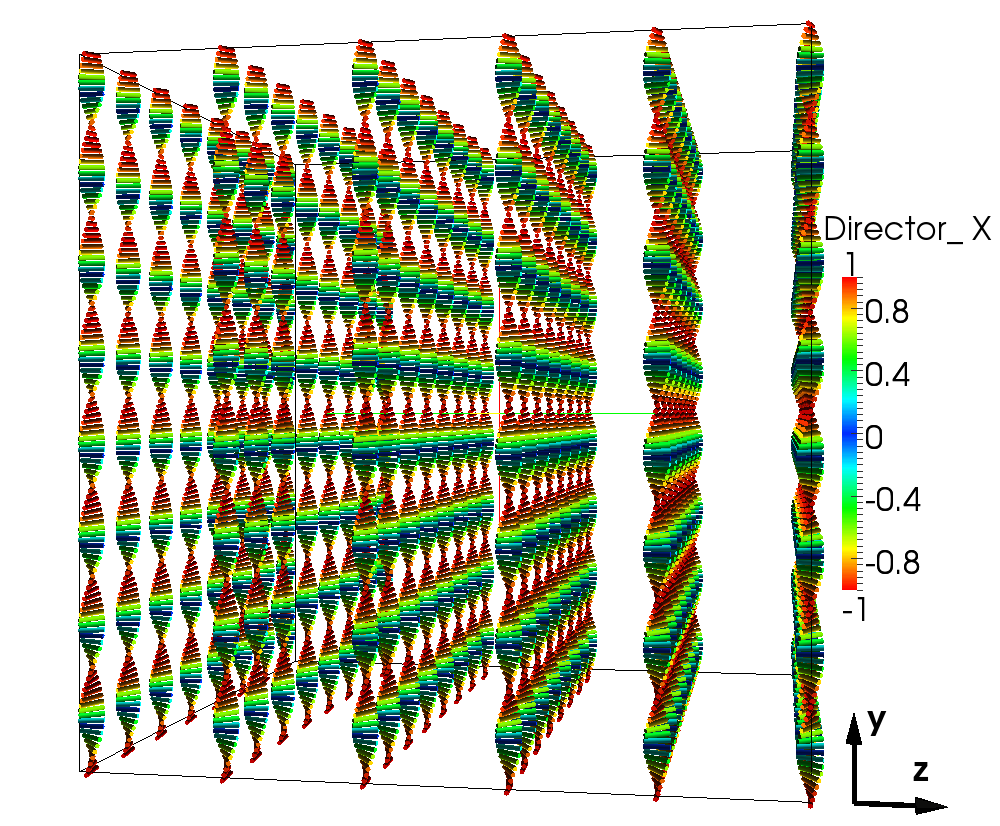
\includegraphics[width=0.45\textwidth]{dir3d+y-200k_run1179.png}
\caption{Flow induced cholesteric state: The orientation of the helix is 
along the gradient direction. The director field is quasi-static during 
the flow, which occurs in 'nematic layers'. For clarity the picture shows 
the director field along the y-direction for selected sites in the x-z-plane.}
\label{cholflow}
\end{figure}



%\clearpage

\section{Conclusions}

In summary, our work constitutes the first simulation of bulk flow behaviour 
of cubic BPs in simple shear flow. Although experimental evidence to support
our results is currently not available, we believe this work can shed some light into the 
flow properties of complex liquid-crystalline phases.
  
We were able to characterise the rheology of cubic BPs and identified 
two different flow regimes for BPII and three different ones in case of BPI. 
Below Ericksen numbers $Er\simeq3$ BPII exhibits weak shear-thinning and 
obeys a power-law.  The BPII disclination network breaks up and reconnects 
in the flow, which leads to a periodically recurring dependence 
of the deviatoric shear stress. The flow-induced conformation look generally
very similar to the quiescent network at equilibrium. 
While being affinely transformed due to the shear flow
the disclination network moves in the vorticity direction. The sense of
motion is directly linked to the helicity of the underlying cholesteric phase.

At larger Ericksen numbers $4\lesssim Er\lesssim 10$ the flowing BPII network 
breaks up in a two-step scenario. First a simple cholesteric helix forms with the helical axis 
in vorticity direction. The flow is in vorticity mode, i.e. as a travelling helical wave. 
At slightly larger shear rates another cholesteric conformation emerges.
However, this time the orientation of the helix is in gradient direction.
The flow is in quasi-nematic layers with static orientation of the directior field. 

Interestingly, BPI shows a flow behaviour that is very different to that of BPII.
This is a direct consequence of the topological differences in both disclination 
network. Below Ericksen numbers $Er<0.4$ the BPI network cannot flow and 
retain a regular appearance. It dissolves eventually into an amorphous network and 
features yield-stress behaviour. The reason is that shortly after the onset of the shearing 
very large stress fluctuations occur. At the lowest shear rates
the contribution of the network to the total deviatoric stress is temporarily 
actually negative during one cycle. These fluctuations destabilise the network and 
eventually trigger its dissolution into an amorphous state with 
dynamic yield stress.

At slightly larger Ericksen numbers $0.4<{\it Er}<8$ shear thinning is 
slightly stronger than for BPII, but BPI does not show simple power-law 
behaviour. 
Instead, it appears BPI kinematically bypasses the large stress fluctuations and 
flows with very complex, periodically recurring flow-induced conformations.
The offset of the network after each cycle is random in magnitude and direction.
However, despite their complex appearance the flow-induced conformations are 
topologically connected to the quiescent BPI and switching off of the 
shear flow often restores a perfect equilibrium.
It is possible to interpret these findings as an instance of 
deterministic rheochaos.

Just as in case of BPII, the BPI network breaks up at larger Ericksen numbers in
a two-step process. First at $10\lesssim\gd\lesssim 15$, it adopts a 
quasi-two-dimensional configuration that is translationally invariant in vorticity direction. 
Then at $16\lesssim Er \lesssim 22$ it forms cholestric helix along the gradient 
direction that emerges from BPII.  
Finally, at $Er\gtrsim30$ (BPI) and $Er\gtrsim10$ (BPII) the configuration
is a flow-aligned nematic state.

% If in two-column mode, this environment will change to single-column
% format so that long equations can be displayed. Use
% sparingly.
%\begin{widetext}
% put long equation here
%\end{widetext}

% figures should be put into the text as floats.
% Use the graphics or graphicx packages (distributed with LaTeX2e)
% and the \includegraphics macro defined in those packages.
% See the LaTeX Graphics Companion by Michel Goosens, Sebastian Rahtz,
% and Frank Mittelbach for instance.
%
% Here is an example of the general form of a figure:
% Fill in the caption in the braces of the \caption{} command. Put the label
% that you will use with \ref{} command in the braces of the \label{} command.
% Use the figure* environment if the figure should span across the
% entire page. There is no need to do explicit centering.

% \begin{figure}
% \includegraphics{}%
% \caption{\label{}}
% \end{figure}

% Surround figure environment with turnpage environment for landscape
% figure
% \begin{turnpage}
% \begin{figure}
% \includegraphics{}%
% \caption{\label{}}
% \end{figure}
% \end{turnpage}

% tables should appear as floats within the text
%
% Here is an example of the general form of a table:
% Fill in the caption in the braces of the \caption{} command. Put the label
% that you will use with \ref{} command in the braces of the \label{} command.
% Insert the column specifiers (l, r, c, d, etc.) in the empty braces of the
% \begin{tabular}{} command.
% The ruledtabular enviroment adds doubled rules to table and sets a
% reasonable default table settings.
% Use the table* environment to get a full-width table in two-column
% Add \usepackage{longtable} and the longtable (or longtable*}
% environment for nicely formatted long tables. Or use the the [H]
% placement option to break a long table (with less control than 
% in longtable).
% \begin{table}%[H] add [H] placement to break table across pages
% \caption{\label{}}
% \begin{ruledtabular}
% \begin{tabular}{}
% Lines of table here ending with \\
% \end{tabular}
% \end{ruledtabular}
% \end{table}

% Surround table environment with turnpage environment for landscape
% table
% \begin{turnpage}
% \begin{table}
% \caption{\label{}}
% \begin{ruledtabular}
% \begin{tabular}{}
% \end{tabular}
% \end{ruledtabular}
% \end{table}
% \end{turnpage}

% Specify following sections are appendices. Use \appendix* if there
% only one appendix.
%\appendix

%\section{}

% If you have acknowledgments, this puts in the proper section head.
\begin{acknowledgments}
We acknowledge support by EPSRC grant nos. EP/E045316 and EP/E030173, 
the MAPPER EU-FP7 project (grant no. RI-261507) and computing time on HECToR.
We thank Peter J. Collings for very stimulating discussions. 
MEC holds a Royal Society Research Professorship.
\end{acknowledgments}

% Create the reference section using BibTeX:
\bibliography{bprheo}

\end{document}
%
% ****** End of file apstemplate.tex ******

